\documentclass[10pt,onecolumn,openright]{book}

% Configure title, author, etc of the thesis in TexFiles/settings.tex

%================================================================%
%  All packages and new commands are treated in an own document  %
%================================================================%
%%=========================================================================%
%%                               Settings                                  %
%%=========================================================================%

%Comment out or remove if it's a Licentiate thesis!
\def\phdThesis{1}

% Important commands for this thesis!
\newcommand{\currentyear}{2024}
\newcommand{\authorname}{Jesus Aguilar Lopez}
\newcommand{\mytitle}{Spoken Language to Irish Sign Language Machine
Translation: A Linguistically Informed Approach}
%\newcommand{\mysubtitle}{With some subtitle if you want it} % Comment out if you don't want a subtitle

\newcommand{\division}{School of Informatics and Cybersecurity}
\newcommand{\researchgroup}{Natural Language Processing group } % Comment out if not applicable


%PHD ONLY
\newcommand{\phdISBN}{xxx-xx-xxxx-xxx-x}
\newcommand{\phdSeriesNumber}{xxxx}
\newcommand{\techReportNumber}{XXXX}


%==============%
% Other common strings, these might need to be changed to follow updated guidelines

%\newcommand{\licISSN}{1652-876X}
%\newcommand{\phdISSN}{0346-718X}

\newcommand{\chalmers}{Technological University Dublin}
\newcommand{\gotuni}{Blanchardstown Campus}
\newcommand{\mydepartment}{School of Informatics and Cybersecurity}
\newcommand{\chalIgu}{\chalmers~\IfItalicsTF{$|\!$}{$|$}~\gotuni} % The \! (negative thin space) is to fix kerning because italics seems to add extra space on the right of the inline math
\newcommand{\chalandgu}{\chalmers~and~\gotuni}

\ifx\phdThesis\undefined
\newcommand{\degreetitle}{Licentiate of Engineering}
\else
\newcommand{\degreetitle}{Doctor of Philosophy}
\fi


%\ifx\phdThesis\undefined
%reportNo is not used for lic anymore, but double check with the intranet.
%in case you need it just uncomment the text in the identifierNoText command.
%\newcommand{\identifierNoText}{%Technical Report No \techReportNumber \\
%ISSN \licISSN\\
%}
%\else
%\newcommand{\identifierNoText}{ISBN \phdISBN\\
%Doktorsavhandlingar vid Chalmers tekniska h\"{o}gskola, Ny serie nr %\phdSeriesNumber .\\
%ISSN \phdISSN\\
%Technical Report No. \techReportNumber \\
%\vspace{1.5cm}
%}
%\fi




%%=========================================================================%
%%                               Settings                                  %
%%=========================================================================%
\setlength{\headheight}{14mm}

% G5 format
\usepackage{geometry}

\ifx\inlagaPage\undefined
% Thesis is paper size G5
\geometry{paperwidth=169mm, paperheight=239mm, inner=28mm,outer=22mm,top=22mm, bottom=18mm}
\else
% Presentation sheet uses paper size A5
\geometry{paperwidth=148mm, paperheight=210mm, inner=25mm,outer=25mm,top=22mm, bottom=18mm}
\fi

%-----------------------Used packages---------------------------------------------------------%
\usepackage{fancyhdr}
\pagestyle{fancy}
\fancyhead[LE,RO]{\thepage}
\fancyhead[RE]{\scriptsize \slshape \leftmark}
\fancyhead[LO]{\scriptsize \slshape \rightmark}
\fancyfoot[C]{}

\setcounter{secnumdepth}{3} \setcounter{tocdepth}{3}

\usepackage[labelformat=simple]{subcaption}
\renewcommand\thesubfigure{(\alph{subfigure})}
\usepackage{graphicx}
\usepackage{url}
%\usepackage{cite}
% \usepackage{multibib}

%\usepackage[english]{babel}
\usepackage[british]{babel} % Using english will cause dates in the bibliography to be mm-dd-yyyy, instead of the more proper dd-mm-yyyy
\usepackage[backend=biber,style=apa,maxcitenames=3,backref=true,language=british]{biblatex} 
%Different styles depending on whether you want numeric/alphabetic citation key
% style=ieee
% style=apa
\addbibresource{references.bib}

\usepackage{amsmath,amssymb,amscd,latexsym,dsfont}
%\usepackage[latin1]{inputenc}
%\usepackage{amsmath}
%\usepackage{amssymb}
%\usepackage{latexsym}
\usepackage{textcomp}
% \usepackage{multirow}
% \usepackage{multicol}
\usepackage{psfrag}
\usepackage{rotating}
%\usepackage{xspace}
%\usepackage{enumerate}
\usepackage{enumitem}
\usepackage{pdflscape}


\usepackage[final]{pdfpages}
\usepackage{xspace}
\usepackage{relsize}

\usepackage{url}
\usepackage{IEEEtrantools}

% \usepackage{fixltx2e}

\usepackage{microtype}

\usepackage{float}

\usepackage{longtable}

\usepackage{setspace}

\usepackage{bbding}

\usepackage{colortbl}

\usepackage{lscape}

\usepackage{rotating}

\usepackage{booktabs}

\usepackage{tabularx}

\usepackage[OT1]{fontenc}

\newtheorem{exmp}{Example}[section]

\renewcommand*\familydefault{\sfdefault}

\usepackage[textsize=tiny,textwidth=20mm,backgroundcolor=orange!70]{todonotes}
\setlength{\marginparwidth}{20mm} % This is so the notes don't get cut out of the page

%----------Some commands you can use-----------%

\newcommand{\figref}[1]{Fig.~\ref{#1}}
\newcommand{\tabref}[1]{Table~\ref{#1}}
\newcommand{\chapref}[1]{Chap.~\ref{#1}}
\newcommand{\secref}[1]{Section~\ref{#1}}
\newcommand{\eqnref}[1]{Equation~\ref{#1}}
\newcommand{\paperref}[1]{Paper~\romannum{#1}}

%use this command to denote figure element that appear inside a figure
\newcommand{\fe}[1]{\textsf{\small #1}}

\newcommand{\p}[1]{\textsf{\small #1}}

\newcommand{\interviewquote}[2]{\begin{quote}
\footnotesize{\emph{``#1'' }} --- \footnotesize{#2}
\end{quote} }



%----------Some commands we need-----------%

\makeatletter
\newcommand*{\IfItalicsTF}{%
  \ifx\f@shape\my@test@it
    \expandafter\@firstoftwo
  \else
    \expandafter\@secondoftwo
  \fi
}
\newcommand*{\my@test@it}{it}
\makeatother


\newcommand{\romannum}[1]{{\uppercase\expandafter{\romannumeral #1\relax}}}

\onehalfspacing

%\linespread{1.0}
% \newcites{ltex}{Appended Publications}
%\addto\captionsenglish{\renewcommand{\figurename}{Fig.}}


%%==============The document begins here
\begin{document}
\frontmatter

%================================================================%
% Auxiliary pages
%================================================================%
%The first three pages. Regulated by the Chalmers/GU layouting guidelines.
%CHECK those to be sure the format is up to date and everything is included!
%================================================================%
%                          First page                            %
%================================================================%

\thispagestyle{empty} %\addtolength{\topmargin}{1cm}
\begin{center}
  \textsc{Thesis for The Degree of \degreetitle}\\
\end{center}

\vspace{4cm}

\begin{center} {\LARGE \textbf{\mytitle}}\\
\ifx\mysubtitle\undefined
\else
  \vspace{4mm}
  \textit{\large\mysubtitle}
\fi
\end{center}

\ifx\mysubtitle\undefined
\vspace{5mm}
\else
\vspace{2mm}
\fi

\begin{center}
\textsc{\large\authorname} \\
\end{center}

\vfill

\begin{center}
\textit{\mydepartment}\\
\textsc{\chalIgu}\\
Dublin, Ireland, \currentyear \\
\end{center}

%================================================================%
%                       Printing page                            %
%================================================================%
\newpage
\thispagestyle{empty}

\vspace{2cm} \noindent \textbf
\mytitle\\
\ifx\mysubtitle\undefined
\else
  \textit{\small\mysubtitle}
  \\
\fi

\noindent
\textsc{\authorname}\\

\vskip 0.5cm\noindent
\copyright \space \authorname,~\currentyear  \\
\noindent
%except where otherwise stated. \\
%All rights reserved. 
\vspace{1cm}


\vfill


%\noindent \identifierNoText

\noindent 
\mydepartment\\
Division of \division\\
\ifx\researchgroup\undefined\else\researchgroup\\\fi
\chalIgu\\
%SE-412 96 Göteborg,\\
%Sweden\\
%Phone: +46(0)31 772 1000

\vskip 1.5cm

%Cover:\\
% If there is a cover image, you should describe it here
%\\

\noindent
%Printed by ... %Chalmers Digitaltryck,\\
Dublin, Ireland \currentyear.


\setcounter{page}{1}

%================================================================%
% Table of contents, list of figures and tables
%================================================================%
\thispagestyle{empty} % To avoid page numbers in blank pages
\cleardoublepage
\thispagestyle{plain}
\tableofcontents 
%\newpage

%If needed, lists of figures and tables
%\listoffigures
%\listoftables
 
%\thispagestyle{empty} % To avoid page numbers in blank pages
%\cleardoublepage

\mainmatter

%================================================================%
% Chapters
%================================================================%
%\thispagestyle{empty} % To avoid page numbers in blank pages
%\cleardoublepage 
\part{Introduction}
\label{part:introduction}
%\thispagestyle{empty}
%\cleardoublepage 
\chapter{Introduction and Background} \label{sec:introduction}


\section{Background}

This research work is focused on creating an architecture of translation from English text to Irish Sign Language (ISL) based on linguistics analysis and computational linguistic approaches to address the challenges of creating a translation system that is efficient in producing lexical information related to ISL.\\

Nowadays, there is an important advance in technology. However, it is not available to everyone. Excluding some groups, generally impaired people, in this case, deaf and hard hearing people. The exclusion leaves deaf and hard-of-hearing individuals at a disadvantage, aggravating the human-to-human communication barrier while suppressing an already under-resourced set of languages further for the estimated 72 million deaf people in the world (Murtagh, I., Nogales, V. U., \& Blat, J.,2022).\\

Deaf people can communicate with each other using sign language, but if a hearing person has to communicate with a deaf person or vice-versa, communication has many barriers. In such cases, a translation process is required, which can translate the hearing person’s spoken language to the sign language of the deaf person and vice-versa.

\newpage


\section{Motivation}

Many deaf and hard-of-hearing individuals rely on sign
language (SL) on a daily basis as a preferred language (Murtagh, I., Moiselle, R., Leeson, L., 2021).
Although nowadays there are significant advances in spoken
language research, current approaches are often neither
linguistically motivated nor tailored to the unique features of
SLs (De Coster, M., Shterionov, D., Van Herreweghe, M. et al., 2023) . Further research and development are necessary to
Enhance Sign Language Machine Translation (SLMT) and bring
it to a similar level as spoken language MT. This research will
endeavour to improve the accuracy and efficiency of SLMT
systems, making them more accessible to the Deaf community
and empowering deaf and hard-of-hearing individuals to
communicate more effectively with the rest of the world.\\


The lack of information and studies about ISL machine translation is a motivating factor. Machine translation (MT) of verbal language (speech/text) has garnered widespread attention over the past 60 years. On the other hand, the computational processing of signed language has unfortunately not received nearly as much attention, resulting in its exclusion from modern language technologies. Furthermore, MT helps to mitigate the needs of interpreters in Ireland since there is a ratio of 1:45 interpreters for deaf people (Leeson and Venturi, 2017). This impact the communication between hearings and deaf people. 

\newpage




\section{Objectives}

\subsection{General objective}

The general objective of this work is to develop a linguistically motivated sign language machine translation (SLMT) avatar that will translate between English (text) and Irish Sign Language (ISL).



\newpage

\section{Hypothesis}

Our hypothesis is that integration of the theory of grammar Rol and Reference Grammar (RRG) is an adequate approach to lead to an accurate and efficient translation.  

\newpage


\section{Research questions}

\subsection{Question 1}
%What grammar theory is suitable for producing ISL lexicon entries?
How a ISL sentence is constructed ?


\subsection{Question 2}
%What is a SL Classifier, and How Do they present themselves or behave?
How to construct a sentence that is robust enough to capture the linguistic phenomena of classifiers in ISL?

\subsection{Question 3}
%How do we create an SL lexicon entry that is robust enough to capture the linguistic phenomena of classifier predicates?
How do a classifier predicate manifest within a ISL sentence?

\subsection{Question 4}
How can we link the SL lexicon entries to the animation interface when generating a ISL sentence?

\newpage

\section{Methodology}

In this section, we discuss the methodology of this research study. We review the data and resources to use.

\subsection{Description of methodology}

For this project the methodology used is the RRG in the development of our
computational linguistic model for ISL. 

In order to represent the translation, we will create a 3D avatar, considering using the following technologies, MakeHuman or Ready Player Me is an open source technology for create an avatar, Blender or Unity as a rendering engine. 

\newpage

%\section{Organization of the research study}

%\subsection{organization}

\newpage


\label{part:literature}
%\thispagestyle{empty}
%\cleardoublepage
\part{Literature review}
\label{part:isl}
%\thispagestyle{empty}
\chapter{Irish Sign Language}


\section{Introduction}

This chapter provides an overview of the literature on Irish Sign Language. Introducing evolution till nowadays, design features of ISL. Providing an account of how ISL is expressed, specifically how signers use the body to communicate and the issues about it. Moreover, it reviews the features of a natural language in terms of linguistics (phonology and morphology) compared to ISL. 

\section{What is a Sign Language?}

Sign Language is a form of communication used by Deaf and hard-hearing people using visual gesture modality that consists of using body gestures with hands, head, shoulders and facial expressions. \cite{vermeerbergen2023} \\
Sign languages are fully formed and consist of distinct vocabularies and grammatical rules. These languages emerge organically within deaf communities and are not influenced or derived from the spoken languages used in their surroundings.(Vermeerbergen, 1997, 2006; Vermeerbergen et al., 2007; Baker et al., 2016). \\

In the past, sign languages were often overlooked in linguistic research. The primary reason for this disregard was the misconception that sign languages were not genuine natural languages. Many believed all deaf people worldwide used a universal, rudimentary system of gestures and pantomime. Additionally, there was a misconception that sign language involved directly translating the spoken language into signs, aligning the signs with the spoken words in content \cite{vermeerbergen2023}.  

However, neither of these assumptions proved accurate, and their falsehoods gradually began to change after the publication of "Sign Language Structure" by the American linguist Stokoe in 1960. This publication had a significant impact, sparking interest in sign linguistics and leading to a steady increase in recognition. Today, while not all linguists and non-linguists fully acknowledge the linguistic status of sign languages, linguistic research into sign languages has established a solid position within various linguistic subdisciplines. One of Stokoe's contributions was emphasising that the signs used in American Sign Language (ASL) should not be considered as indivisible units but rather as composed of smaller components that distinguish meaning. (Vermeerbergen, Herreweghe, 2023).

While spoken languages use the oral-aural modality, sign languages exploit the visual-gestural modality. As a result, sign languages draw on their specific linguistic mechanisms (Meier, 2002). Signers use visible articulators to communicate: the hands, face, torso and other body parts are needed for communication production, whereas the eyes (and writings, in the case of tactile sign languages used by deafblind people) are required to perceive a signed message. Signs consist of manual and non-manual parameters or building blocks. Manual parameters include hand shape, orientation, movement and location (Baker et al., 2016). Non-manual parameters are movements of the face and body, e.g. mouth gestures and facial expressions (Vermeerbergen, 1997; Baker et al., 2016).

Collectively, the five sign language parameters – shape, Place of Articulation (where the sign is formed), Movement, Orientation (the hand's position about the Place of Articulation), and Non-manual features (body and facial actions) – function in a manner analogous of the components found in spoken languages: cavities, articulators, and features. Although these parameters have different content, they undergo operations that exhibit resemblances to the processes seen in spoken languages, and they are collectively referred to as phonemic feature groups within sign languages. However, it's crucial to recognise that these overarching similarities are tempered by significant differences arising from the influences of modality and iconicity on the system. (Pfau, Steinbach and Woll, 2012) \\
 In the early stages of modern research, the focus on sign languages highlighted the fundamental structural similarities they share with spoken languages. However, recent research has shifted towards recognising systematic typological distinctions (Goldin-Meadow and Brentari 2017 provide a comprehensive overview of this evolving research emphasis). These differences primarily emerge from the interplay between language structure and modality. Phonological and morphological arrangements vary due to sign languages' stronger connection between form and meaning (iconicity or visual motivation) than spoken languages. Sign languages also leverage the characteristics of their articulators (the hands being the primary ones, alongside non-manual articulators like the torso, head, face, eyes, and mouth) and the distinctive attributes of visual and auditory perceptual systems. This space utilisation serves grammatical and discourse functions, resulting in syntactic structures characterised by extensive simultaneity, while spoken languages tend to favour linearity and affixation processes. (Woll, 2023)\\


 \subsection{Sign language phonology}

 Phonetics is the field of study that focuses on speech sounds produced by humans and the organs involved in their production. Phoneticians investigate the process of combining speech sounds to form words and how these sounds interact during speech. Also, phoneticians ask questions such as: How many different sounds do languages use? How does sound travel through the air? How do the ears register it? How can we measure speech? Phoneticians also work on how to describe any sound precisely. Then, in 1888, a phonetic inventory called the International Phonetic Alphabet (IPA) was created, which contains the sounds of human speech represented by a symbol. The IPA was created using the Roman alphabet to write down the sounds of any spoken language. The IPA has been revised to incorporate the new findings. The latest revision was in 2005. \\

Sandler and Lillo-Martin (2006) define phonology as "the
level of linguistic structure that organises the medium through which language
is transmitted." \\
 In addition, Johnston and Schembri (2007) say that phonology is "the study of how sounds are organised into the words and phrases of different languages. Although phonetics and phonology both
originally referred to the study of sounds in spoken language, they are also
used by sign language researchers to refer to the physical properties of signs
(signed language phonetics) and how signs are created from smaller
formational units (signed language phonology)." \\

 According to Woll (2023), from Stokoe's groundbreaking research on American Sign Language (ASL) in 1960, linguists have perceived signs as complex combinations of concurrent handshape configuration, articulation location, and movement. This encompasses the trajectory through the signing space and the internal joint movements within the hand. Each component is considered phonological because modifying them can create a distinct minimal pair. Consequently, in British Sign Language (BSL), words like AFTERNOON1 and ORDER contrast only in Handshape, while AFTERNOON and NAME2 differ solely in location, and AFTERNOON and TWO-HUNDRED solely in movement1. Since Stokoe's initial framework, there have been significant adjustments, particularly in acknowledging the importance of movement sequences and holds within a sign's structure (Liddell and Johnson 1989). Additionally, it's been proposed that these sublexical parameters resemble features more than phonemes. Nevertheless, despite these developments, Stokoe's model has endured as the foundational depiction of sign language phonology.

 \subsection{Sign language morphology}

 The smallest meaningful units of a language are known as morphemes
(Bloomfield, 1933). Morphemes are used in the language to create the larger
units we call words and signs and modify existing terms and gestures.\\

Research conducted crosslinguistic on sign languages from 1970 has discovered that these languages exhibit a simultaneous morphological structure and share similar grammatical categories. Additionally, sign language morphology has two different types: simultaneous and sequential (Aronof, Meir and Sandler, 2012). 

Words within a language are tasked with multiple functions. They serve as tools for language users to denote any concept they wish to communicate, whether it's an object, a thought, an occurrence, or a characteristic. Additionally, words need to interact with one another, enabling users to communicate information by expressing opinions, descriptions, or details about specific subjects or individuals. To accomplish the initial objective, it's essential to establish methods for generating fresh words when denoting novel concepts is necessary. As for the secondary objective, when merged to shape more extensive constructs, words must be capable of undertaking diverse functions like serving as subjects, predicates, or modifiers. Certain words could be tailored for specific roles, and languages might incorporate mechanisms for crafting words for particular functions. (Pfau, Steinbach and Woll, 2012)\\

Sign languages possess words, standardised entities of form-meaning connection akin to spoken languages. These entities hold cognitive significance for their users (Zeshan 2002). They consist of smaller linguistic components and exhibit a dual pattern structure (Stokoe 1960). They demonstrate particular phonological arrangements and are influenced by specific phonological limitations (Sandler 1999; consult Chapter 3, Phonology). Typically, these words in sign language are denoted as "signs."

Three indications propose reasons for the valuable insights that sign language morphology can provide into the mechanics of the grammatical system. Firstly, an inherent iconic foundation is present in all natural sign languages. The second significant aspect is the many methods employed to create intricate words within these languages. Lastly, universal principles governing organisation and structure, which impact spoken language morphology, also sway sign language despite its iconic origin. Thus, morphology is the apparent intersection where iconically driven sign language forms meet linguistic structuring.(Sandler and Lillo-Martin, 2006) \\

Two prevalent, if not universally present, characteristics of sign language morphology include a substantial employment of compounding, whether sequentially or simultaneously, and a diverse array of inflexion types involving modifications in position, speed, repetition, and non-manual attributes. Many sign languages exhibit a considerable degree of inflexion (Zeshan 2003; Sandler and Lillo-Martin 2006; Lutalo-Kiingi 2014), with instances where complete sentences are constructed from a single, highly inflected sign. Signs can undergo inflexion to indicate grammatical aspects such as a person, number, location, aspect, manner, and mood, contingent upon the sign's category (Sutton-Spence and Woll 1999).\\

Sign language morphology often becomes evident by blending meaningful handshapes, positions, and motions. In the context of derivational morphology, handshape alterations can represent numerical values. For instance, within BSL, expressions like "N weeks," "N o'clock," and "N years old" are formed using standardised patterns of location and movement, with the handshape conveying the specific number (Woll and Sutton-Spence, 2023). 


\section{Evolution of Irish Sign Language}

 The history of Irish Sign Language relates to Deaf education and educational policy (Leeson and Saeed,2012). The first recorded school for deaf students in Ireland was founded in 1816. Over the years, various educational institutions were established, including the Claremont Institute, which initially taught a Protestant doctrine but later shifted with the advent of Catholic institutions. In 1846, the Catholic Institution for the Education of the Deaf and Dumb was established, inspired by a similar institution in France (Leeson and Saeed, 2012). The Dominican Sisters managed St Mary's School for Deaf Girls and adapted the French methodical signing system for English teaching. In 1849, the Christian Brothers opened a school for Deaf boys. St Joseph's School in Cabra became the last major institution for Deaf education in the 19th century (McDonnell 1979). On the 20th century, Mary Immaculate School for Deaf Children (Beechpark School) was established in 1956 following a request from Archbishop Charles McQuaid (Matthews 1996b).\\

\subsection{What is Irish Sign Language?}

Irish Sign Language is a visual-gestural language using the signer's hands, torso, face, head, shoulders and eyes. The signs are expressed in the three-dimensional space known as 'signing space'. See Figure 2.1. (Leeson and Saeed, 2012) \\

Irish Sign Language (ISL) is used by an estimated 5,000 Deaf people in the Republic of Ireland and some 1,500 signers in Northern Ireland. It is neither Irish (Gaeilge) on the hands nor English in manual form. (Leeson and Saeed, 2012)

According to Lesson and Saeed (2012), The critical universal features across languages include arbitrariness, iconicity, the duality of articulation, semanticity, creativity, and structural dependence. Leeson and Saeed (2012) say that the arbitrariness of the sign is a feature that receives a lot of attention in the literature. Arbitrariness suggests no necessary link between the word and the object it denotes. Iconicity is about the relationship between the form of the sign and the referent it refers to.
\\
Duality of articulation is the organisation of language at two levels, meaningless or meaningful units. For example, phonemes are typically useless in isolation but are significant when combined as morphemes. For example, indicative signs in ISL must comprise a handshape, a location, a movement and an orientation. Without these combined, we have phonological components of characters but not meaningful morphemes. Thus, a handshape or a place by itself is simply phonetic. Semanticity denotes the use of symbols that refer to objects and actions. For example, the literal sign BOIL is expressed in neutral space in ISL. At the same time, the idiomatic expression BOIL+c (I'm boiling (angry)) consists of the same manual sign BOIL, with one modification: the place of articulation moves from neutral space to the signer's body (stomach area). 
\\
Now terms of creativity in a linguistic sense refers to our capacity to produce and understand an indefinite number of sentences, our ability to create from finite means (for example, a limited number of sounds/handshapes that are possible in a language, a finite pattern of rules, etc.) and an infinite number of utterances. Irish Sign Language is a language that is evolving, and as such, as new themes become relevant to daily life, signs are developed to express new concepts. (Leeson, Saeed, 2012)
\\
Yet another feature of human language is structural dependence: language is arranged in structured chunks, not simple linear sequences. This impacts word order issues, on the one hand, and how we interpret broader lines of meaning, on the other (for example, the scope of negation marking or the identification of a topic). (Leeson, Saeed, 2012)


\section{Phonology of ISL}

In signed languages, phonology focuses on analysing and breaking down the continuous movements of the signer's hands, body, and facial expressions. Specific elements like handshapes are extracted from this gestural flow through phonetic analysis, identifying their linguistic significance. There is no consensus on the inventory of a phonetic alphabet for ISL. For instance, Ó Baoill and Matthews (2000) have identified sixty-six handshapes. See fig. \\
Describing the phonology of a signed language involves exploring
how phonological units are formed by combining handshapes
and other phonetic features and trying to discover the rules that govern how
these units are combined to form higher-level elements like words. (Leeson, Saaed, 2012) \\

The most significant research work in sign languages was made by Stokoe in 1960 in his research paper, where Stokoe used linguistic principles to analyse ASL and identified that it is composed of three main linguistic components: hand configurations, movements, and placement. This analysis of sign language structure laid the foundation for recognising sign languages as real languages.\\

In addition, Battison (1978) suggested adding a parameter of orientation, 
the spatial relationship of the palm and fingers to the signer's body.\\

\subsection{Manual Features} 

The first works in sign language phonology where were described the parameters of the signs, such as hand configuration,
movement, and place of articulation (Stokoe 1960; Stokoe et al. 1965; Klima
and Bellugi 1979).

The manual features consist of Handshape, which pertains to how the hand or hands are configured. Location refers to the placement of the hands concerning the signer's body or the signing space. Movement involves the hands and arms' paths while signing and may encompass internal finger and thumb movements. The orientation of the palm plays a crucial role in phonology and can result in minimal pairs (Leeson and Saaed, 2012).

\subsubsection{Location}

Stokoe (1960) called the parameter location a tab, and he defined a set of members named primes, where location primes include face, nose, and trunk. 
According to research on British Sign Language, Brennan et al. (1984) identify five distinct spatial locations: the head (including the neck), the trunk, the arms, the hands and the area in front of the signer's body. They subdivide each location into specific tabs. For example, the head area is reported to have ten tabs, and each is allocated because certain signs differ only in their position on or near the head. So, in BSL, the eye, ear, nose, mouth and forehead are considered separate tabs. Sandler (1989) introduced the idea of utilising setting features to precisely define specific positions within the primary place of articulation. Per her proposal, these setting features can represent the movements occurring within these central articulatory locations.

ISL has the exact spatial locations as BSL, identifying minimal pairs based on tab differences.

\subsubsection{Handshapes}

A handshape is one of the manual features used to articulate a sign. Handshapes can be said to represent one of the phonetic possibilities of a signed language, and the use of particular handshapes is linguistically determined (Leeson and Saaed, 2012). \\
However, the human hand can adopt an extensive range of alternative forms. It can be clenched into a fist or stretched with fingers spread apart or touching. The writing is flexible at the wrist, allowing the fingers to flex at the knuckles or joints. The thumb can be extended, aligned with the fingers, placed across the palm, or within a closed fist. The index, middle, ring, and little fingers may be extended, curved, or positioned in contact with one another. As we will explore further, despite the multitude of potential hand configurations that can be generated, each specific sign language tends to employ only a limited set of handshapes to construct signs in its core vocabulary. (Johnston and Schembri, 2007)

The size of the handshape inventory may differ from one sign language to another, but there.
There is not as much variation as in the sound inventories of spoken languages.
The study of many sign languages has resulted in lists of frequently occurring handshapes (Baker, 2016).

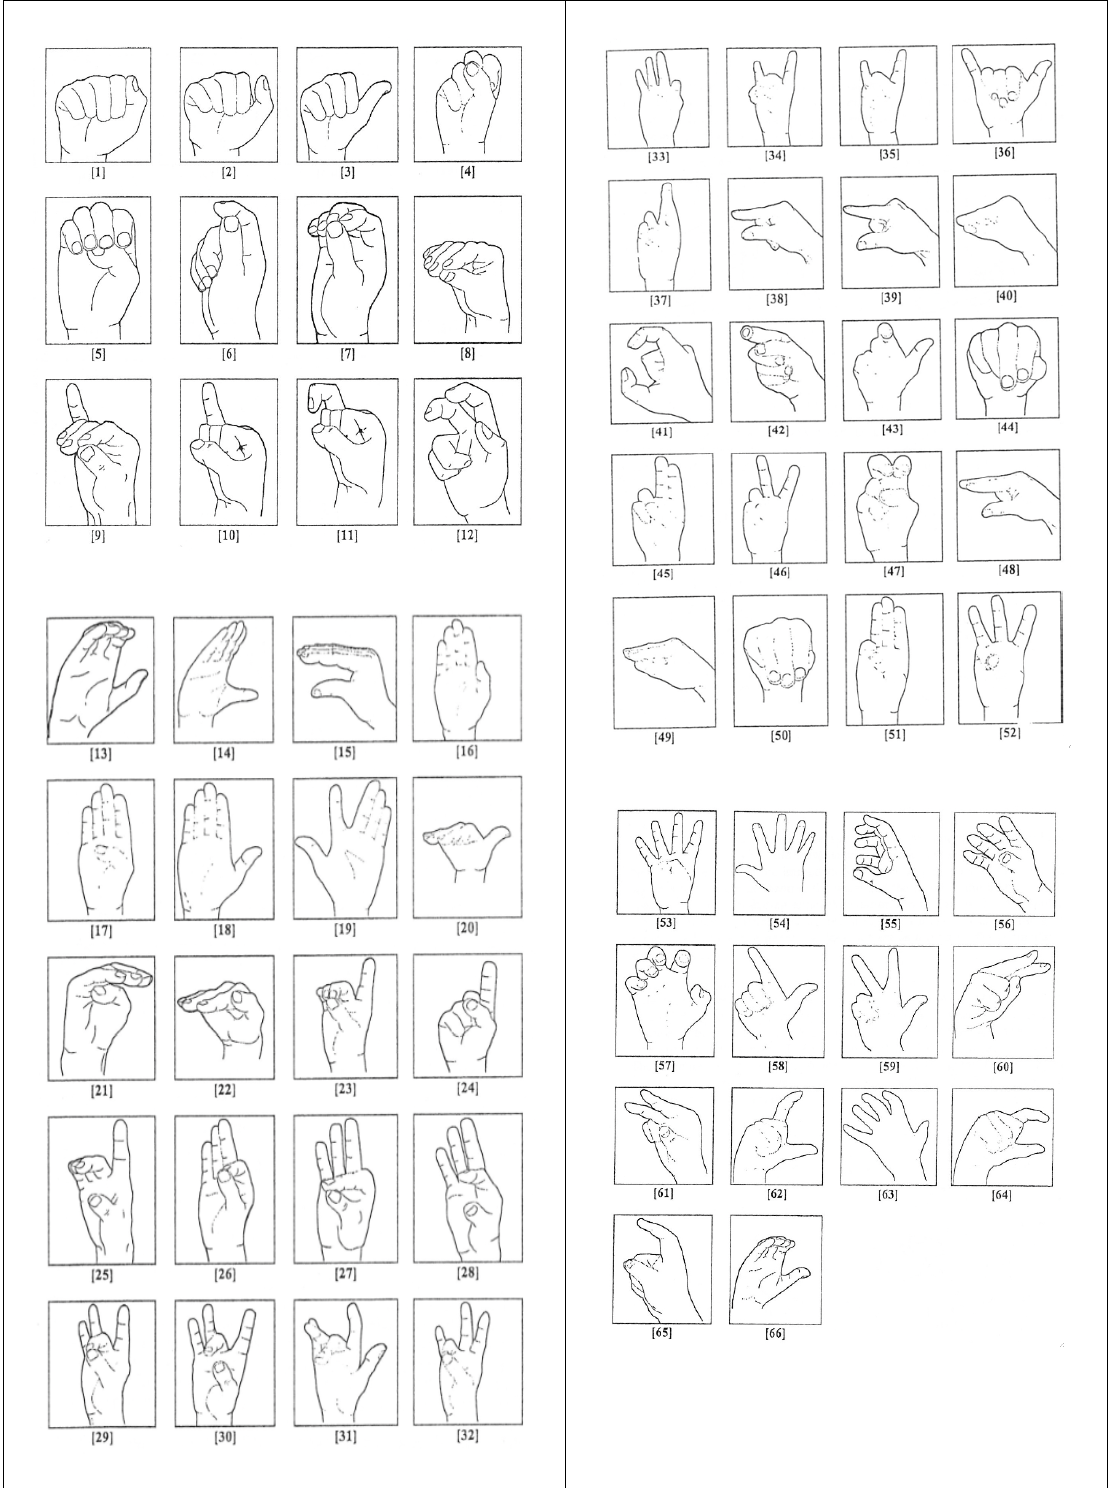
\includegraphics[width=\textwidth]{figures/handshapes.png}

\subsubsection{Movement}

Among the three fundamental components, movement emerges as possibly the most intricate. The hand can traverse away from the body, towards it, upwards, downwards, back and forth, in curved paths like arcs, circles, or spirals. Hand-shape alterations or adjustments in the palm and fingers' orientation could occur. While certain signs employ straightforward motions, others may manifest as intricate amalgamations of diverse movement patterns. If the sign is executed with the palm of the dominant hand positioned toward the signer, additional factors such as the tempo, duration, repetition rate, stress, and the manner of sign production come into play in shaping signs in Auslan (Johnston, 1989a). \\

The feature analysis of movement offered by Friedman (1977) includes four fundamental features: interaction, contact, direction and manner. Also, according to Baker (2016), movement has been considered one of the phonological parameters since Stokoe's phonological description of ASL. There are two types of movements: path and local. The first is the movements of the entire hand. The latter are the movements of the fingers and the wrist (hand-internal movements and orientation changes) 


\subsubsection{Orientation}

Initially, there was a heated debate regarding whether orientation should be considered a fundamental parameter for description. In 1977, Friedman advocated for its inclusion, suggesting that exposure should be defined for each handshape to determine the hand direction of the body. On the other hand, in 1978, Stokoe argued against its necessity. However, Brennan et al. (1984) decided to include the orientation parameter in their analysis based on two key factors. First, orientation can be the sole distinguishing feature between two lexical signs. Second, previous transcription systems that excluded orientation were proven inadequate.
Sandler (1989) proposed categorising the orientation parameter within a node termed 'hand configuration,' referred to as an articulator by Hulst and Kooij (2021). This categorisation was inspired by assimilation patterns observed in lexicalised compounds within both ASL and Israeli Sign Language (ISL), as earlier demonstrated by Sandler in 1987. These patterns revealed that orientation could propagate independently or combine with the overall handshape.

In Irish Sign Language, orientation is crucial in distinguishing between different sets of minimal pairs—for example, the following image (Leeson and Saeed, 2012).

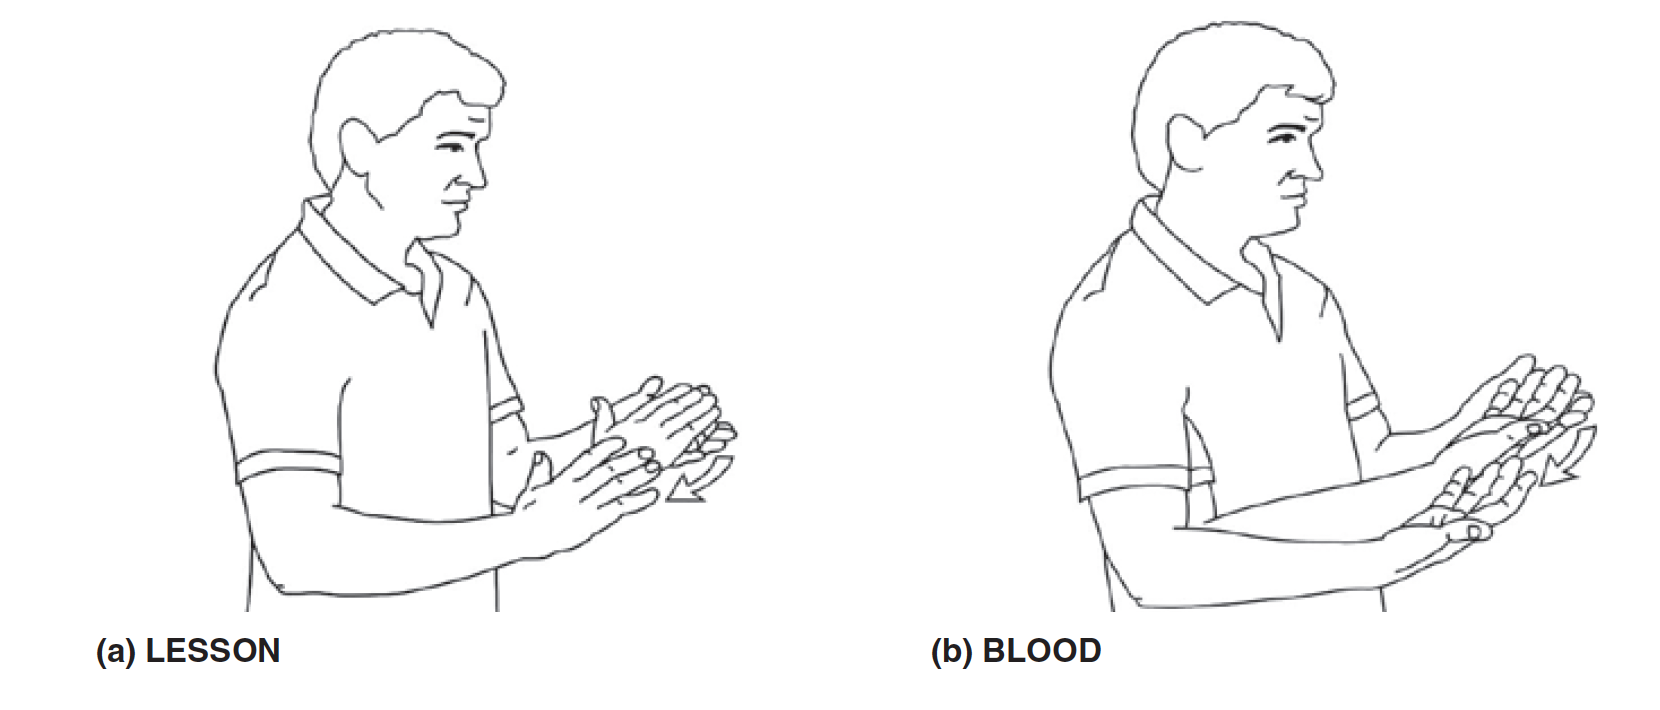
\includegraphics[width=\textwidth]{figures/orientation.png}


\subsection{Non-manual features}

Research on sign languages has revealed the contribution to the meaning of non-manual markers such as facial expressions, head movements, bodily posture and mouthing. 

In signed languages, non-manual signs involve eye, head, body movements, facial expressions, lip movements, and mouth gestures (Johnston and Schembri, 2007).

Mouthings are derived from a spoken language and are evidence of the contact between English and Irish Sign Language. 
Mouth gestures, \textcite{sutton2007mouthings} points out that these are idiomatic gestures of the mouth and cannot be traced back to a spoken language. 

The types of non-manual features used by ISL signers are given in Figure 2.1.

According to \textcite{sutton2007mouthings}, although we commonly associate signed languages with manual communication, they convey crucial linguistic information through non-manual channels, such as the mouth. Studies on sign languages have demonstrated the significance of non-manual elements like facial expressions, head movements, body posture, and mouthing in contributing to the overall meaning of the signed messages.

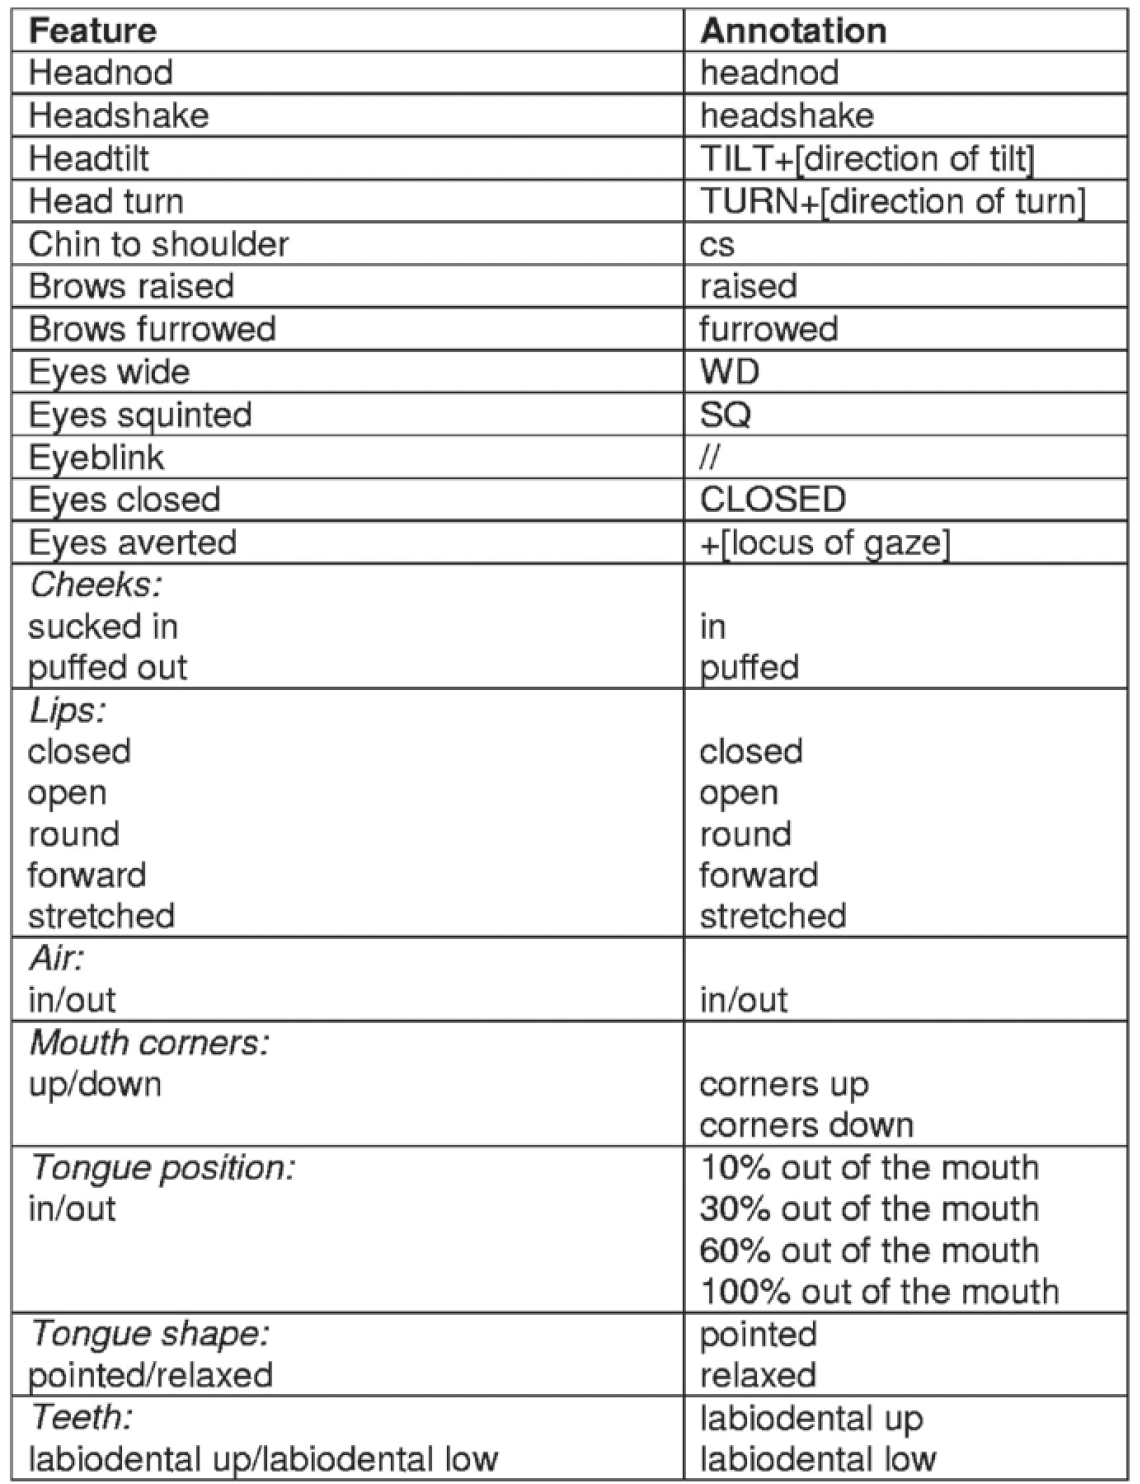
\includegraphics[width=\textwidth]{figures/nm.png}
\captionof{figure}{Extracted from \parencite{leeson2012}:80 Section 4.6, Articulatory descriptors for non-manual features in Irish Sign Language}


\section{Morphology of ISL}

\subsubsection{Morphemes}

As Bloomfield (1933) described, a morpheme is the most elementary meaningful entity within a language. These are the meaningful components of a word that cannot be broken down any further without losing their significance.

Morphemes like bikes and shoes are considered to be 'free morphemes'. In contrast, morphemes like –s (in shoes), -er (in biker) and -ing (ingoing) cannot stand alone as words, but they also carry meaning. Units like these are called 'bound morphemes'. Signed languages also exhibit free and bound morphemes. For example, ISL morphemes function as words in their own right, like HOUSE, GIRL, SISTER and HAVE. (Leeson, Saeed, 2012) \\
Leeson and Saeed follow Brenan in using the term 'word' in a general sense to incorporate spoken, signed and written language. We will use the term 'sign' when referring only to signed languages, considering that 'signs' are equivalent to 'words' in terms of grammatical role. 


\subsubsection{Locus}

A locus denotes a designated spatial point where an entity has been established, and this locus serves as a reference point for subsequent mentions within the discourse. Notably, a locus need not be confined to a specific physical location within the signing space; it can also possess a 3-D function, symbolising a spatial position. Signers employ classifier predicates to depict real-world entities, positioning them in relation to one another in a manner that mirrors their real-world configurations, a spatial arrangement commonly known as topographical space (Liddell, 1990). Also, signers can designate an entity by either producing a lexical sign or a classifier at a specific spatial location or initially signing and directing attention through pointing or eye gaze toward a particular area in space. (Emmorey,  1996) 

The employment of syntactic space is to convey non-locative syntactic and semantic information using loci. Within this context, a locus is characterised as a "random, abstract point" within space that serves as a reference for a particular entity without the exact position within the signing space being of significant relevance. (Vermerbergen and Herrewedge, 2023)

In sign languages, certain verb signs are adjusted to spatially indicate the subjects or objects of the verb, which can be categorised into two types: currently present and not. Regarding non-present referents, signers establish specific spatial locations known as loci (Padden, 1988a; Poizner, Klima, and Bellugi, 1987). When a verb agrees with the subject and object, it typically employs the referential space by starting at the locus representing the subject and ending at the locus representing the object. (Sandler and Lillo-Martin, 2006). 


\subsubsection{Compounds} 


A prevalent word-formation process extensively employed in American Sign Language (ASL), ISL and various other sign languages is compounding, as extensively documented in studies such as those by Klima and Bellugi (1979), Bellugi and Newkirk (1981) and Wallin (1983) in the context of Swedish Sign Language.  \\




\section{The ISL Lexicon}


As users of a language, people possess the knowledge of phonological, morphological, and syntactic principles governing their language, in addition to a substantial repository of individual words or signs. This compilation of known words or symbols is called the lexicon, and each word or sign within this compilation is denoted as a lexical item. (Vali and Lucas, 2001)

The lexicon of a particular language comprises a compilation of elements present within the language. These elements are essential for a speaker to be familiar with as they represent arbitrary signs, often displaying unpredictability. While many of these elements consist of individual words, the lexicon encompasses more extensive entities such as idioms and potentially even smaller components like affixes (Aronoff and Anshen, 2001).

Several researchers, notably Padden (1998), Brentari and Padden (2001), who have predominantly focused on American Sign Language (ASL), have postulated a division within the lexicon. According to their proposals, this division comprises two primary components. The initial component encompasses the complete inventory of native sign vocabulary, commonly termed the lexicon. The secondary component, the non-native lexicon, primarily emerges from interactions with the English language. \\

In their Auslan sign language lexicon research, Johnston and Schembri (2009) introduced a fundamental distinction between the native and non-native lexicon. The native lexicon within Auslan comprises signs that have evolved within the framework of Auslan itself, adhering to a predefined set of nativisation constraints. These nativisation constraints encompass various criteria, including conditions related to symmetry, dominance, and a predisposition for signs to be monosyllabic. Non-native forms contain lexical items that take the form of fingerspelled representations of English words. A parallel distinction is drawn by Brentari and Padden (2001) within the context of the ASL lexicon. They define the non-native lexicon as comprising "signs said to be borrowed from English such as initialised signs and loan signs derived from fingerspelling" (ibid.). Consequently, the non-native lexicon encompasses all signs arising from language contact. An alternative term used to describe the core native lexicon of a sign language is the frozen or established lexicon (Johnston and Schembri, 2009)  

After understanding various perspectives regarding the lexicon in diverse sign languages, let's focus on discussing the lexicon, specifically ISL.

Leeson and Saeed (2012) emphasised a crucial conceptual distinction first introduced by Brennan (1992) within the framework of British Sign Language (BSL). This distinction revolves around segmenting the lexicon into two primary facets: the "established" and the "productive" components. 

The lexicon of Irish Sign Language (ISL) undergoes a multifaceted influence from various sources. These encompass lexical borrowings drawn from British Sign Language (BSL) and French Sign Language, in addition to influences stemming from the English language through mechanisms such as mouthed, initialised, fingerspelled, and Cued Speech elements. Furthermore, the lexicon is subject to gestural components, such as gestures associated with object manipulation, which can be regarded as substrates contributing to the lexicalisation of certain signs. ISL presents free and bound morphemes within its linguistic structure like other sign languages. (Leeson, Saeed, and Grehan, 2015)\\


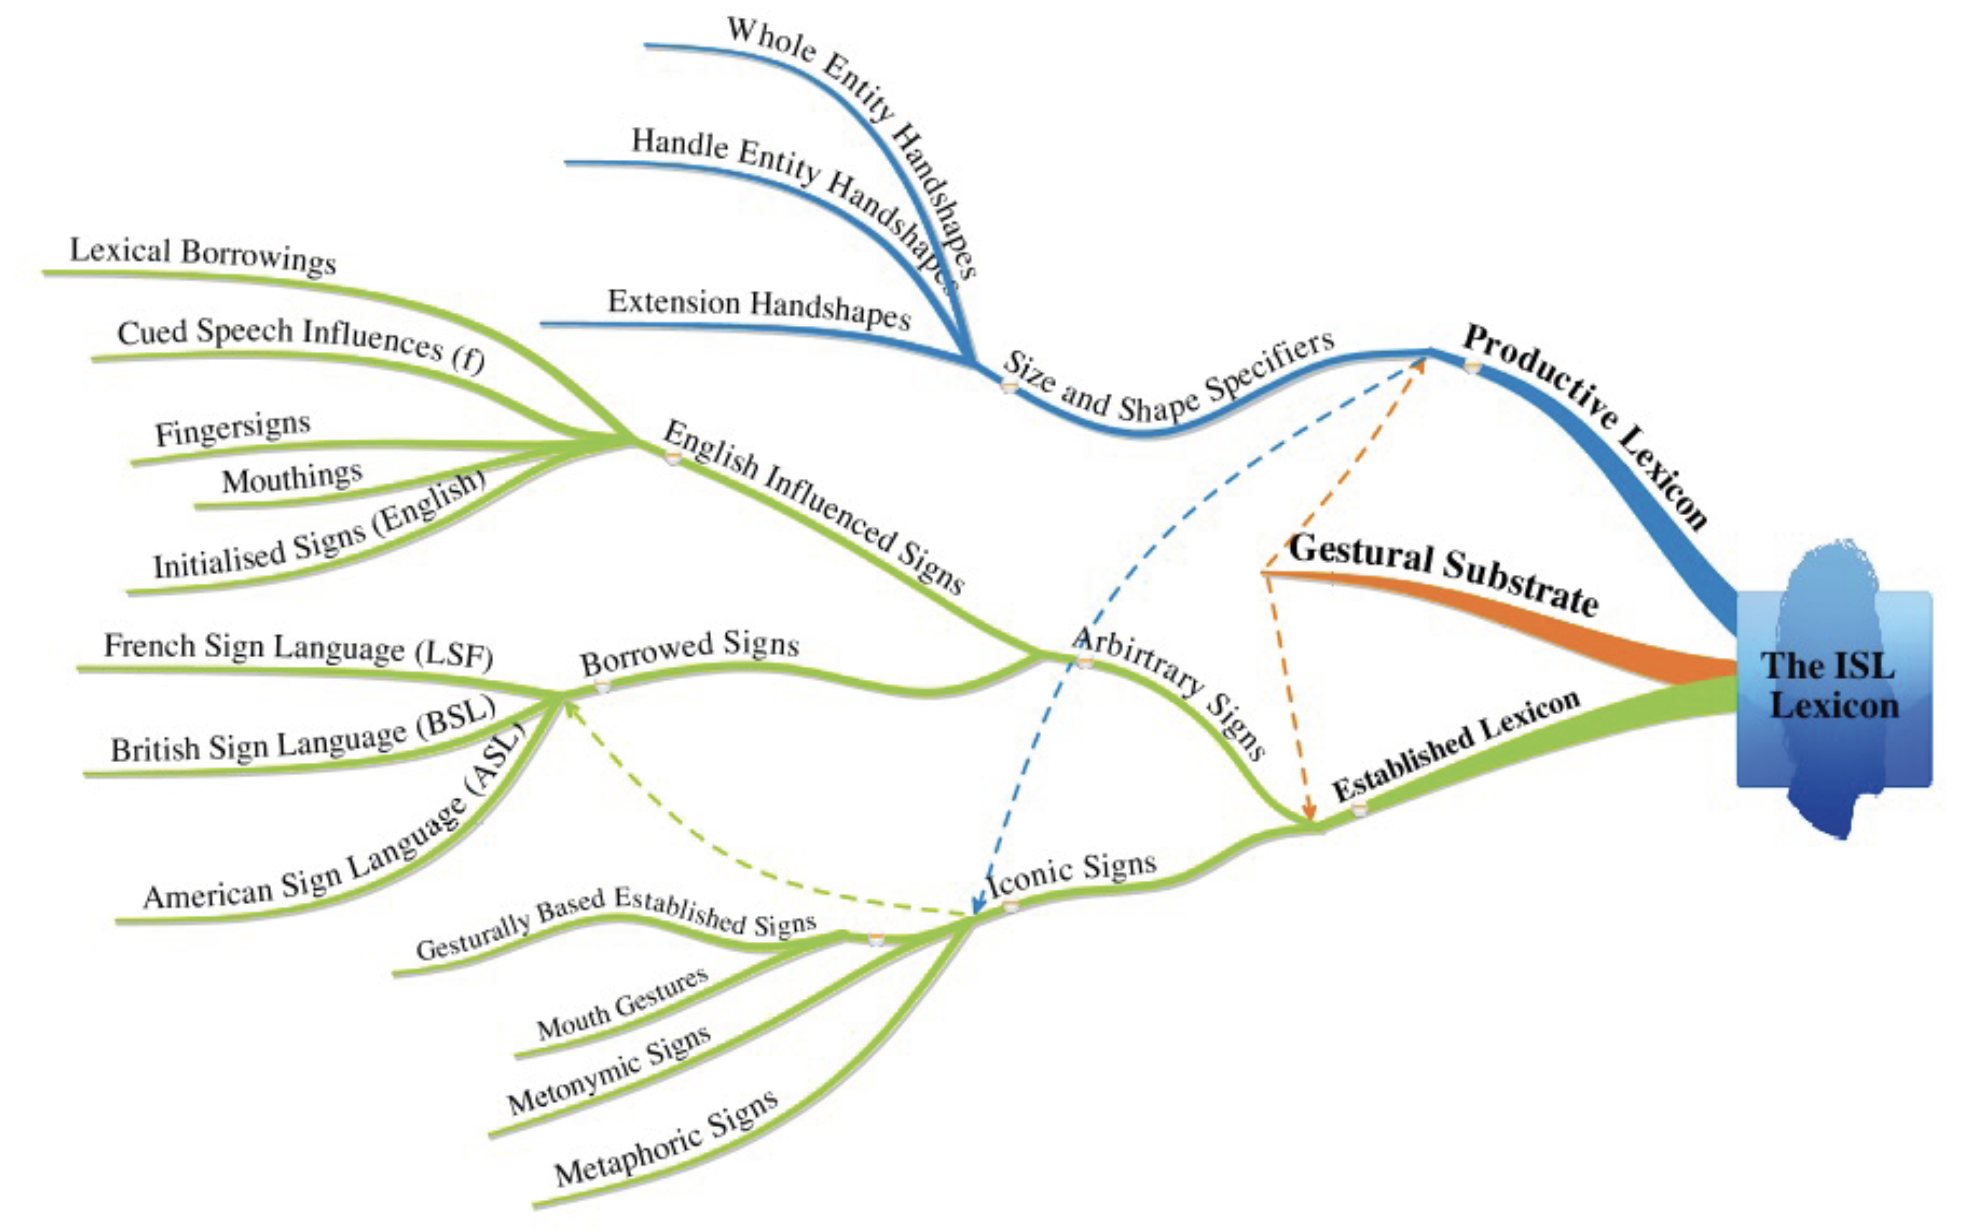
\includegraphics[width=\textwidth]{figures/lexicon.png}
\captionof{figure}{Extracted from \parencite{leeson2012}:127 Section 6.2, The ISL Lexicon}



\subsection{Stablished ISL Lexicon}

The established lexicon of ISL encompasses a variety of signs, both arbitrary and iconic. This includes signs that English has influenced, British Sign Language, French Sign Language, and more recently, American Sign Language. Certain iconic signs might have origins in gestures, often appearing as metonymic forms. Some of these signs are accompanied by mouth gestures, which have become conventionally linked to specific lexical items, particularly those associated with gender-specific concepts. (Leeson and Saeed, 2012)

\subsection{Productive ISL Lexicon}

In the productive lexicon, gesture is a fundamental building block for multiple functional elements. These elements have undergone standardisation, elevating them to a position of linguistic significance. Utilising size and shape specifiers, commonly called classifier handshapes, assumes a prominent role within this particular category. (Leeson and Saeed, 2012)










\label{part:classifiers}
%\thispagestyle{empty} % To avoid page numbers in blank pages
\chapter{Classifiers}
In this chapter we provide a background of classifiers in ISL. We first provide an 
account of classifiers in spoken language and sign language. We delve into  the 
morphological, grammatical details, handshapes conveyed by classifiers within ISL as 
described in literature. 


\section{What is a classifier?}

Classifiers are commonly found in nearly all the sign languages examined so far. They 
constitute a thoroughly investigated area within the field of sign language 
linguistics. Nevertheless, there is still considerable ongoing discussion regarding 
various aspects of these elements \parencite{zwitserlood2012}.
The beginning of research into classifiers within sign languages coincided with the 
renewed interest in studying classifiers in spoken languages. \parencite{zwitserlood2012}. 

Having defined classifiers as morphemes that indicate a semantic class of items 
belong. Various analyses of classifiers have been presented in the literature on the 
linguistics of spoken language \parencite{morgan2007}. 

To mention a remarkable work made by Allan (1977). He proposed four distinct 
classifiers languages. Sign language classifiers align with one of these classifiers 
called predicate classifiers. To demonstrate this, they made the comparison of 
structures in Navajo and ASL; this comparison is based on a misinterpretation of 
classificatory verbs of Navajo (Engberg-Pedersen 1993; Schembri 2001; Zwitserlood 
1996, 2003). \textcite{vermeerbergen2023} stated that the previous comparison 
and due to various factors, including the issues discussed extensively by \textcite{schembri2003}, several sign linguists have opposed the interpretation of the handshape 
within what is commonly referred to as "classifier constructions" as classifiers. 
Moreover, the concept that every constituent element of these constructions is 
separate, can be listed, and is explicitly delineated within the grammar of specific 
sign languages, each possessing morphemic status (as proposed by Supalla in 1982), 
has also been subject to scrutiny and scepticism.

According to \textcite{zwitserlood2012}, classifiers are primarily conveyed through specific 
arrangements of the manual articulator and represent entities by signifying their 
prominent and distinctive attributes. 

\textcite{morgan2007} mention three types of verbs (plain, agreeing, and spatial 
verbs) where classifiers fall in the category of spatial verbs. Spatial verb 
classification comprises the verbs of movement and location, often called "classifier 
verbs." So, classifier verbs describe essential details regarding the path, 
trajectory, speed, and spatial location of the depicted action or movement. Then, 
classifier predicates are predicates of direction or location \parencite{zwitserlood2012}.

In Australian sign language (Auslan),\textcite{schembri1996structure} shows that Auslan has similar 
constructions identified in other sign languages. This category was called 
polycomponential verbs (PVs) of motion, location, and visual-geometric description.
Schembri points out that the significant element represented by handshape in PVs 
has commonly been defined as a classifier morpheme. This is due to the apparent 
variation in handshape selection based on the prominent attributes of the referent, 
particularly its shape.

\textcite{valli2001linguistics} defined a classifier in ASL as a handshape combined 
with location, orientation, movement, and nonmanual signals to form a predicate. For 
their part \textcite{valli2001linguistics}, use the English sentence \textit{The car drove past 
}as an example of a classifier. Here, the sign car is used, followed by a sign with a 
3 handshape, moving from right to left in front of the signer, with the palm facing 
in. A sign with the same handshape can be used to talk about the movement of a boat or a bicycle.
\newpage

\subsection{Classifier types}

In terms of categorisation, Zwitzerlood 2012 analyses the classification provided 
by Supalla (1982, 1986), which divided the ASL classifiers into five types: 

\begin{table}[H]
    \centering  
\begin{tabular}{ |p{4cm}|p{7cm}|}
\hline
\multicolumn{2}{|c|}{Categorization of classifiers} \\
\hline
 Classifiers & Description \\
\hline
Semantic Classifiers & Represent nouns by some semantic characteristic of their 
referents (e.g., belonging to the class of humans, animals, or vehicles) \\ \hline
Size and Shape Specifiers (SASSes) & Denote nouns according to the visual geometric 
features of their referents. 
SASSes come in two subtypes:
\begin{itemize}
\item Static SASSes: Consist of a handshape (or combination of two hands) that 
indicates the size/shape of an entity.
\item Tracing SASSes: These have a movement of the hand(s) that outlines an entity’s 
size/shape and in which the shape of the manual articulator denotes the 
dimensionality of that entity.
\end{itemize}
\\ \hline
Instrumental Classifiers & Instrumental comes in two types:
 Hand classifiers, in which the hand represents a hand that holds and/or manipulates 
 another entity.
 Tool classifiers, in which the hand represents a tool that is being manipulated.\\ 
 \hline
Bodypart Classifiers   & Body parts represent themselves (e.g., hands, eyes) or limbs 
(e.g., hands, feet). \\ \hline
Body Classifier & The body of the signer represents an animate entity.  \\
\hline
\end{tabular}
\caption{ASL Classifiers}
\label{tab:asl_classifiers}
\end{table}


Schembri (1996, 1998) categorize PVs into three subcategories: verbs of motion and location, handling, and visual-geometric description. Also, \textcite{zwitserlood2012} mentioned that most researchers no longer view the body classifier as a classifier; instead, they see it as a mechanism for shifting references (Engberg-Pedersen, 1995; Morgan and Woll, 2003). Additionally, \textcite{zwitserlood2012}  argues that  SASSes do not belong to the classifiers domain for the following reasons: 
A mere hand configuration does not express them, and they also need the tracing movement to indicate the shape of the referent.
They cannot be combined with verbs of motion. 
They denote specific shape information (all shapes can be outlined, from square to star-shaped to Italy-shaped). They can be used in various syntactic contexts: they appear as nouns, adjectives, and (ad)verbs and do not seem to be used anaphorically.\\

According to \cite{kimmelman2020}, the following classifier types are well-known:


\begin{table}[H]
\centering 
\begin{tabular}{ |p{4cm}|p{7cm}|}
\hline
\multicolumn{2}{|c|}{\textbf{Classifiers categories}} \\
\hline
 \textbf{Classifiers} & \textbf{Description} \\
\hline
Whole-entity classifiers & Whole-entity classifiers refer to whole objects whose movement or location is described by the predicate. They can be further divided into:
\begin{itemize}
    \item Semantic classifiers refer to a semantic class of objects (humans, trees, cars). 
    \item Size-and-shape specifiers refer to some formal characteristics of the contour of objects (thin objects, round objects, etc.). 
\end{itemize}\\
\hline
Body-part classifiers & Where the hand refers to a body part: a hand, a head, a leg, a tail, etc.\\ 
\hline
Handling classifier & the hand refers to a hand or another manipulator handling some object.\\ 
\hline
\end{tabular}
\caption{Classifiers categories}
\label{tab:asl_classifiers}
\end{table}

The literature researchers recognise two primary classifier categories: Whole Entity 
classifiers and Handling classifiers. Whole Entity classifiers are typically utilised 
in verbs that convey the movement of a referent, its spatial placement, or its 
presence within a given space. In such instances, these classifiers directly depict 
the referent. Conversely, Handling classifiers find their application in verbs that 
portray the manipulated motion or the act of holding a referent \parencite{zwitserlood2012}. 
Also, Zwiterslood mentions a relation between the type of classifier and the verb 
transitivity. In the same way, Benedicto and Brentari (2004) furthermore assert that 
the classifier that is attached to the verb is also responsible for its 
(in)transitivity: a Handling Classifier turns a (basically intransitive) verb into a 
transitive verb.

Regarding the classifier's form, denotation and variation, \textcite{zwitserlood2012} states 
that signers in most sign languages can employ multiple classifiers when representing 
an entity. This allows them to emphasise a specific, distinct characteristic of the 
entity or, conversely, to de-emphasise it.

In terms of classifiers verbs, Supalla (1982) and subsequent studies (Benedicto and 
Brentari, 2004; Chang et al., 2005 Cuxac, 2003; Glück and Pfau, 1998, 1999; 
Zwitserlood, 2003, 2008) proposes the perspective that classifiers function as 
agreement markers or proforms for the referent concerning the verb.

\subsection{Classifiers in ISL}

As mentioned before, predicate classifiers are aligned to signed languages. According 
to that, Brennan (1992) identifies six types of classifier handshapes: semantic, size 
and shape, tracing, instrumental, handling and touch. Based on Brennan's work, 
McDonnell (1996) categorised the predicate classifiers into four categories: Whole 
entity-CL, Extension-CL, Handle entity-CL, and Body-CL. 

\subsubsection{The whole entity-CL stems}

This type of classifier stems from the hand configuration, which usually signifies a 
complete entity. McDonnell (1996) suggests these stems can be paired with the same 
types of movements in ISL, specifically MOVE, BE-LOCATED, and EXIST. Leeson and Saeed 
(2012) identify the following subcategories of whole entity-CLs: Semantic-CL stems, 
which describe entities based on their semantic characteristics (e.g., those that are 
+animate). Size and shape-CL stems represent entities in terms of their shape (e.g., 
rectangular) or their dimensions (e.g., 'two-dimensional object').
McDonnell (ibid) defines the semantic-CL as the ‘multiple entity-CL handshape’. This 
is identifiable as the ‘5-hand/s’; typically, the multiple entity-CL handshapes 
signifies entities as members of large groups.

\subsubsection{Extension-CL stems}

Extension-CL are those stems that trace size and shape the entities they refer to. 
These stems can be paired only with EXTEND movements. 

\subsubsection{Handle Entity-CL Stems}

Handle entity-CL stems denote, with the configuration of the hand, how an actor 
moves, touches or uses an object or part of an object rather than the object as a 
whole. These stems combine the following ISL movements: MOVE, BE-LOCATED and EXIST 
(Leeson and Saeed 2012) \cite{leeson2012}.

\subsubsection{Body-CL stems}

Body-CL stems use the signer's body as an independent articulator to refer to a 
single animate entity. This classifier in ISL refers to the actual body of the 
animate entity rather than the semantic category of the entity's shape. Also, Leeson 
and Saeed (2012) \cite{leeson2012} suggest using these stems when the signer's body functions similarly 
to the way that handshape functions in two-handed configurations.



\subsubsection{Terminology of classifiers}

Schembri (2003), in his terminology analysis of handshape units for describing these 
complex constructions in various sign languages, shows a diversity of terms. For 
instance, in  Australia, they are called classifiers signs or classifiers (Bernal, 
1997 and Branson et al., 1995). Other regions and countries have different names, 
such as classifier verbs or verbs of motion and location (Supalla, 1986, 1990), 
and classifier predicates ( Frishberg, 1975. Kegl and Schley, 1986. Corazza, 1990. Schick, 1987, 1990. Smith, 1990, Valli 
and Lucas, 1995. ), spatially descriptive signs (DeMatteo, 1977), spatial-locative predicates (as mentioned by Liddell and 
Johnson, 1987), polymorphemic predicates (as discussed by Collins-Ahlgren, 1990, and Wallin, 
1990), polysynthetic signs (Takkinen, 1996, and Wallin, 1996, 1998), productive signs 
(Brennan, 1992. Vermeerbergen, 1996 and  Wallin, 1998), polycomponential signs (Slobin et al., 2001), Polymorphemic verbs 
(as described by Engberg-Pedersen, 1993. Schembri, 2003). Depicting verbs (Liddell, 2003; Dudis, 2004) and depicting signs 
(Johnston and Schembri, 2007. Ferrara, 2012).\\

\textcite{schembri2003} chose the term polycomponential verb following the work of Slobin et al. (2000) to refer to 
the classifiers rather than other authors' alternatives. Because of the following 
reasons: First, he stated that the allegation that these forms include classifier 
morphemes is debatable. Second, analyzing these as a multimorphemic is tricky 
(Cogill,1999).
% add text about monomorphemes 
According to \textcite{schembri2003}, This lack of consensus on categorising 
handshape units within PVs may reflect the inherent complexities in linguistic 
descriptions of these forms. Various researchers have proposed markedly different 
analyses regarding delineating the subclasses of handshape units in PVs. \\

\begin{table}[H]
 \centering  
 \begin{tabular}{ |p{2cm}|p{3cm}|p{3cm}|p{3cm}|}
\hline
\multicolumn{4}{|c|}{\textbf{Classification of Classifiers in Signed Languages}} \\
\hline
 \textbf{Author} & \textbf{Entity Handshape Units} & \textbf{Handle Handshape Units} 
 & \textbf{SASS Handshape Units} \\
 \hline
 Supalla & Static SASSes, semantic, bodypart, some instrument classifiers & Some 
 instrument classifiers & Non-static SASSes \\
 \hline
 McDonald & Some x-type of object classifiers & Handle x-type of object & 
 Some x-type of object \\
 \hline
 Shepard-Kegl & Shape/object classifiers & Handling classifiers & - \\
 \hline
 Johnston & Substitutors/proforms & Some manipulators & Some manipulators \\
 \hline
 Corazza  & Surface, some grab, perimeter and some quantity (?) classifiers
 & Some grab classifiers & Descriptive, some perimeter and some quantity (?) 
 classifiers \\ 
 \hline
 Brennan & Semantic classifiers, some SASSes & Handling, instrumental and
touch classifiers & Tracing classifiers and some SASSes \\
\hline
Schick & Class classifiers, some SASSes & Handle classifiers & Some SASSes \\
\hline
Engberg-Pedersen & Whole entity stems, some limb stems & Handle stems and some limb 
stems & Extension stems \\
\hline
Liddell \& Johnson & Whole entity, surface, on-surface classifiers and some
extent (?) classifiers & Instrumental classifiers &  Depth and width,
perimeter-shape and some extent (?) classifiers \\
\hline
Zwitserlood & Object & Handle & - \\
\hline
\end{tabular}
\caption{Classifiers in Signed Languages taken from \parencite{schembri2003}:10}
\label{tab:classifiers_signed_languages}
\end{table}


\section{Depicting verbs}

Liddell pioneered a novel perspective on classifier constructions, reimagining them as depicting signs, distinct from fully lexical signs due to their unique characteristic of "depicting certain aspects of their meanings" (Liddell, 2003:261). Liddell posits that these signs possess a blend of both descriptive and depictive qualities. In his work, Liddell (ibid) demonstrates that signers can employ partial lexical classifier constructions and/or constructed action to craft topographical real-space blends. On the one hand, signers can craft depicting blends, manifesting as small-scale representations of the event space they intend to convey in the sign space right before them \parencite{beukeleers2022show}.\\

The method of depiction enables individuals to graphically convey the sensory attributes of an object, encompassing its appearance, sound, or texture (Clark, 1996, 2016, 2019; Enfield, 2009; Dingemanse, 2011, 2014, 2015, 2017; Ferrara and Hodge, 2018; Hsu, 2021). Speakers and signers then construct a tangible representation of the object in the immediate present, amalgamating diverse elements representing the objects within the depicted scenario. Depictions are not subject to decryption; instead, they engage the faculty of imagination in the audience, prompting them to envision how the object appears, sounds, or feels (Clark, 1996, 2016, 2019; Enfield, 2009; Dingemanse, 2015; Ferrara and Hodge, 2018). The method of depicting primarily hinges on the utilization of iconic P-signs, such as manual iconic gestures (McNeill, 1992; Kendon, 2004), classifier constructions (Liddell, 2003 for ASL; Johnston and Schembri, 2007, 2010; Ferrara, 2012 for Auslan), and gestural enactment (e.g., Metzger, 1995; Liddell, 2003 for ASL; Cormier et al., 2015 for BSL; McNeill, 1992; Clark, 1996, 2016; Kendon, 2004; Ferrara and Johnston, 2014; Stukenbrock, 2014; Stec et al., 2016 for spoken languages).\\

Expanding Liddell (2003), Dudis (2007) introduces the term "depiction" to elucidate the visually symbolic mapping of semantic elements in signed languages. Dudis posits the existence of additional components within these iconic representations, including the subject (self), vantage point, and temporal progression. Dudis makes a crucial distinction between depicting and non-depicting verbs, emphasizing that depicting verbs vividly portray the events they encapsulate. Signers possess the ability to depict an experiencing self through various means, such as constructed dialogue, constructed action, or handling classifiers. These depictions can either inhabit the life-sized representation or be intricately linked with the self, though not necessarily occupying life-sized space (Stone and Russell, 2016).

Furthermore, Dudis (ibid)  suggests that an event can be depicted without any representation of the self, utilizing techniques for describing an event or concrete object within generic space, event space, real space, or blended space (Stone and Russell, 2016). \\

Depicting verbs can be divided into fundamental conceptual elements, encompassing a figure or a dynamic or stationary entity, background or context against which the figure operates, the specific movement or location, and the course and manner of that movement (Schembri 2003; Taub and Galvan 2001). These components of Depicting Verbs find expression through semantic/entity classifier handshapes, such as "3" representing vehicles in American Sign Language (ASL), or size-and-shape-specific (SASS) handshapes like "F" or "C" to delineate cylindrical objects. Interactions and transitions between these elements are indicated by these handshapes (Brentari, Coppola, Jung, and Goldin-Meadow 2013; Kantor 1980; Schembri 2003; Schick 1990; Taub and Galvan 2001) (Beal-Alvarez, Trussell (2015) \\


 \textcite{beukeleers2022show} stated that signers possess diverse semiotic tools for conveying meaning. Additionally, they challenge the conventional belief that the primary role of a classifier construction, commonly referred to as a depicting sign, is consistently centered on depiction. Their argument proposes that these constructions find their most insightful analysis when examined within the specific context of their use. Signers can employ them for varying degrees of describing, indicating, and depicting meaning.\\


Depicting Verbs aren't subjective; their meanings remain fluid. Unlike static symbols, which can adopt iconic or arbitrary roles, Depicting Verbs maintains an intrinsic connection between their structure and significance. The handshapes within them can symbolize properties of the object or shape they represent or the characteristics of hands as they interact with an entity. Furthermore, the positions and orientations of the hands correspond to the locations and orientations of the things they refer to or the boundaries thereof. At the same time, the gestures mirror real-world motions or the hand's movement when tracing an object \parencite{beuzeville2006visual}.


%\cleardoublepage
\label{part:avatar}
%\thispagestyle{empty} % To avoid page numbers in blank pages
\chapter{Sign language animation}

In this chapter, we will review the state of the art about signing language 
animation using 3D avatars...

\section{Sign language animation}

Sign language avatars promise to become an indispensable and inclusive reservoir of natural language communication for the signing deaf community. However, developing top-tier avatars demands substantial commitments in terms of time and financial resources. Crafting these high-quality avatars poses a formidable engineering challenge \cite{quandt2020teaching}.


Specific requirements must be satisfied within the avatar file to animate any avatar. These prerequisites include a mesh, a skeleton, a texture, and a collection of morph targets if facial animation is necessary. The mesh 
serves as the outward visual representation of the avatar and, in conjunction with 
the texture, defines the avatar's optical characteristics. The skeleton, though 
imperceptible in the software, consists of interconnected bones, each linked to the 
vertices within the mesh. Consequently, altering the rotation of any bone within 
the skeleton leads to corresponding movements in the mesh vertices connected to it. 
The morph targets, also known as blend shapes, play a crucial role in deforming the 
static mesh. They modify the area around the mouth and jaw for 
speech synchronization and to manipulate the cheeks, eyelids, eyebrows, and 
forehead to convey various facial expressions \cite{jennings2010requirements}.

JASigning is a synthetic animation system for deaf signing, written in Java, that 
has been developed at UEA, taking as input avatar-independent Gestural SiGML 
(Signing Gesture Markup Language) \parencite{elliott2004overview, 
elliott2008linguistic} and producing output motion data for any avatar. SiGML is an 
XML form of HamNoSys (Hamburg Notation System) (Prillwitz et al., 1989; Hanke, 
2004). Animgen uses that (Kennaway, Glauert, Zwitserlood, 2007) To generate 
Signing animation. To achieve this, JASigning requires additional information that 
cannot be obtained from the standard information above and must be provided in 
separate files \cite{jennings2010requirements}.

For the JASigning software, four avatar definition files effectively define each. 
ARP signing avatar. The first of these contains binary data, the other three are
XML: Main Avatar Definition, ASD  Avatar Standard Description,  Animgen Configuration Data, Nonmanuals.

\textbf{Main Avatar Definition} 

\textbf{Vertex list}

A list of vertices representing the mesh defining the avatar's shape, with texture coordinates and vertex normals for each.

\textbf{Texture map}
Defines the appearance of the avatar.

\textbf{skeleton}
The skeleton structure fits within the mesh. It must include all bone names used by 
Animgen.

\textbf{Mesh-to-Skeleton Attachment Data}

This data is a list of links between vertices in the mesh and
the bone(s) that will animate them, with a weight for the influence
of each bone. A maximum of 4 links per vertex is
permitted, with a preferred maximum of 3. The weights of
all links to a vertex must sum to 1.0. This follows standard
industry practice for this data type, as more than four links
to a vertex make weight calculations very complex.\\


\section{Ways to generate an Avatar}

Generating signing avatars through motion capture recordings of native signers can yield significantly more naturalistic results than avatars constructed solely from computer-generated models. Nevertheless, it's essential to acknowledge that the creation of motion-captured avatars demands a considerably higher level of manual labor and presents limitations in automation and the ability to iteratively generate new content compared to avatars generated using computational algorithms \parencite{quandt2020teaching}.


\section{Sign language synthesis}

Sign and utterance synthesis are fundamentally distinct processes 
within sign language technology. Sign synthesis involves the 
creation of skeletal animations for individual signs, focusing on 
isolated linguistic units. In contrast, utterance synthesis 
encompasses the animation of entire sign language sentences, 
necessitating a deeper understanding of sign language linguistics 
and involving distinct mechanisms compared to generating isolated 
signs. To achieve coherent sign language communication, it is 
imperative to consider sign language grammar, ensuring that the 
generated utterances maintain consistency and fidelity to the 
linguistic rules and structure of the specific sign language in 
question \parencite{naert2020survey}.

\subsection{Isolated sign synthesis}

There are two distinct linguistic approaches to animating signing avatars in sign language (SL). The first parametric approach operates at a phonological level and primarily synthesizes isolated signs. This approach focuses on the specific phonological parameters of signs. The second approach concentrates on the sign inflection mechanisms, addressing the more variable and fluid aspects of sign language at a linguistic level. This latter approach is especially relevant during the synthesis of utterances, where the context and fluidity of speech play a significant role \parencite{naert2020survey}.

\subsection{The parametric approach}


To create signs, sign languages use multiple components, such as 
hand configuration, placement, movement, and orientation 
\parencite{naert2020survey}. Unlike vocal languages that construct 
words through a linear sequence of phonemes, sign languages operate 
on both simultaneous and sequential levels. This unique feature of 
utilizing various elements simultaneously is why sign languages are 
described as multilinear. This multilinear nature allows for a rich 
and complex form of communication 
\parencite{sallandre2007simultaneity}.\\

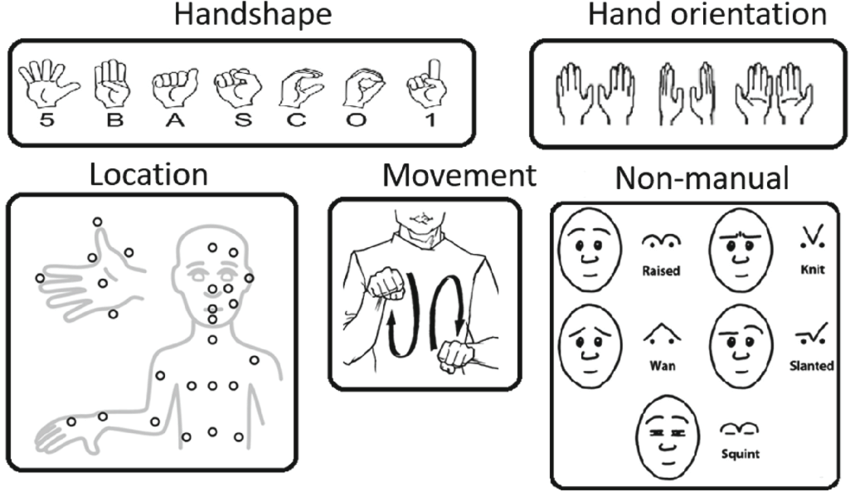
\includegraphics[width=\textwidth]{figures/signcomponents.png}
\captionof{figure}{Extract from \textcite{signlanguagerecogn} Five components of signs in sign language }


The parametric approach to sign language involves constructing signs 
by setting specific values for various phonological parameters and 
combining these into a single virtual character. The combination of 
its parameters uniquely defines each sign. This method focuses on 
creating posters with stable characteristics, ensuring consistency and 
clarity in the language \parencite{naert2020survey}.




\section{Representations of signs}

 For isolated signs, typically synthesized using a parametric approach, this representation needs to emphasize both the structure of the sign and the values of its phonological elements during its production. The spatiotemporal nature of sign languages, which involves space and time dimensions, makes the exhaustive representation of signs challenging. This complexity requires collaboration between experts in linguistics and computer animation. The goal is to accurately capture sign language's dynamic and multifaceted nature, encompassing the physical movements and the linguistic principles underlying them \parencite{naert2020survey}.

 \textcite{naert2020survey} mention three ways of signs representation used in the study of signs: visual representations, gloss representation, parametric notation, and writing systems. In Table 1, there is a comparison of the different sign representations. 

 \subsection{Visual representations}

Visual representations convey ideas, information, or data through a visual format. In this case, to represent signs. According to \textcite{naert2020survey}, the process involves representing signs on a 2D canvas, aiming to be as accurate as possible to the symbol used in sign language since signs involve movements in three-dimensional space and time. Drawings and video recordings are two typical ways of visual sign representations.\\

\subsubsection{Drawings}

Drawings represent the signs on a 2-D canvas by being faithful to the actual sign.
Signs are motions specified both in the 3D space and in time: in a drawing, using arrows and different types of contour (e.g., dotted line or fine line) allows for a partial representation of those dimensions on a 2D paper (See fig. ). However, this schematic representation depends on the user's interpretation and the artist's skill. Drawings are an ambiguous representation that often needs to be clarified with annotations \parencite{naert2020survey}.\\

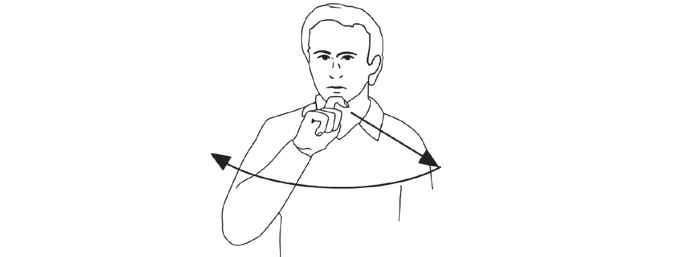
\includegraphics[width=\textwidth]{figures/drawing-isl.jpg}
\captionof{figure}{Extract from from McDonnell (1996) Drawing}



\subsubsection{Videos}

Videos, once produced, are static, meaning they cannot be altered or modified post-production. Additionally, the inability to anonymize individuals in videos is a crucial concern in sign language representation, as the face plays an integral role in meaning through expressions and mouth shapes. The facial component of sign language is essential for complete communication \parencite{kipp2011assessing}. Also, videos are good for capturing the dynamics of sign language. Still, they have disadvantages, including flattening the depth of information, imposing a specific viewpoint on the viewer, and omitting spatial details. Like drawings, their format and limitations render them unsuitable for representing signs in an automated animation engine, which requires a more adaptable and detailed form of representation \parencite{naert2020survey}.

\subsection{Parametric Notation}

\subsubsection{Stokoe}

Stokoe identified three key linguistic elements in his research: the configuration of the hand, hand placement, and hand motion (see section 2.2 for details). Stokoe's notation system represents American Sign Language (ASL) signs. In this system, the sign location is termed 'tabula' or TAB, the configuration of the hand is known as 'designator' or DEZ, and the hand motion is referred to as 'signature' or SIG. These components are each defined using a specific set of symbols \parencite{stokoe2005sign}.

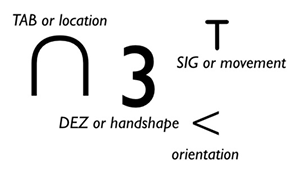
\includegraphics[width=\textwidth]{figures/stokoe-notation.PNG}
\captionof{figure}{Extract from Julie A. Hochgesang for Linguistics 101 at Gallaudet University, 2007}

\subsubsection{HamNoSys}

The Hamburg Notation System for Sign Languages (HamNoSys) is based on the Stokoe notation system, developed by Stokoe in 1960, which was an alphabetic system for describing the sublexical parameters - location, hand configuration (primarily handshape), and movement - of American Sign Language signs. HamNoSys extends this approach, providing an alphabetic system for representing signs, primarily at a phonetic level \parencite{prillwitz1989hamnosys}. 

The parameters of a sign are documented in a specific sequence: first, the symmetry operator, followed by nonmanual components, then hand shape, hand position, location, and finally, movement \parencite{kaur2014hamnosys}.




\subsubsection{SLPA}

The Sign Language Phonetic Annotation (SLPA) framework uses the Posture-Detention-Transition-Shift (PDTS) classification to analyze sign language. It categorizes segments or timing units based on two-timing characteristics: the static/dynamic nature and the transient/deliberate quality of motion. Static segments maintain certain sign language components (like hand configuration, orientation, placement, and non-manual features) unchanged for a period, while dynamic segments mark a transition between static ones \parencite{naert2020survey}. The transient/deliberate quality affects the duration of these segments. SLPA identifies four types of timing units: Posture (static and transient), Detention (static and deliberate), Transform (dynamic and transient), and Shift (dynamic and deliberate). To transcribe a sign, SLPA uses a table format with timing units in columns and articulatory components in rows \parencite{johnson2011segmental}.

\subsubsection{SignWriting}

The SIGNWRITING system is a method for documenting deaf sign languages using a collection of intuitive, graphical-schematic symbols. These symbols and straightforward rules for their combination enable the representation of signs. Due to its graphical nature, SIGNWRITING requires properly encoding its symbols for digital applications. This encoding is essential for storing and processing sign language documents on computers and integrating written sign languages into interactive elements of computer program interfaces \parencite{da2003signwriting}.

\subsection{Scripting language}


\subsubsection{SWML}

The SIGNWRITING MARKUP LANGUAGE (SWML) is an XML-based language designed to facilitate interoperability among systems that process sign languages using SignWriting. SWML can represent SIGNWRITING texts and dictionaries created by programs like SIGNWRITER and SW-EDIT \parencite{da2003signwriting}.

A signbox, which represents a sign, contains the same information as its SignWriting transcription. However, it shares SignWriting's limitations, including ambiguities in hand placement and time management \parencite{naert2020survey}.


\subsubsection{SiGML}

SiGML (Signing Gesture Markup Language) is an XML dialect created for detailing sign language sequences for depiction by a virtual human (VH) signer or avatar. It is closely modeled on the HamNoSys notation, originally developed for transcribing human signing. Like HamNoSys, SiGML describes sign language at the phonetic level. Its scope and role are focused on this aspect, though it differs in other respects \parencite{glauert2011extending}.

SiGML, like HamNoSys, breaks down the description of a sign into a structured format. In its manual part, it represents features like hand shape, orientation, location, and movement. This movement category encompasses not only changes in location but also alterations in hand shape and orientation \parencite{glauert2011extending}.

Developed under the European projects ViSiCAST and eSIGN, which aim to enhance Deaf access to information \parencite{kennaway2003experience}, this language was created to animate virtual signers. Consequently, it allows for more detailed specifications in aspects like timing and precise orientations in SiGML, features that are not as explicitly detailed in HamNoSys \parencite{naert2020survey}. The PDTS classification, developed by Johnson and Liddell, was integrated into an extended version of SiGML \parencite{glauert2011extending}, enhancing the language with explicit timing control, synchronization of elementary motions, and detailed direction specifications in various contexts. This addition positions it as one of the most advanced sign language specifications available for sign language synthesis \parencite{naert2020survey}.

\subsubsection{QualGest}

\textcite{lebourque1999high} defined QualGest, a
high-level specification language dedicated to French Sign Language (LSF) that takes into
account the four manual parameters (hand configuration, place-
ment, motion and orientation), called gestems.

QualGest (Qualitative Gestures specification) system is a \textcite{lebourque1999high} proposal that includes a spatial representation around the signer and a set of movement primitives, hand configurations, and orientations. These elements are combined to describe a gesture, which comprises components that can occur sequentially or in parallel. At a more detailed level, various sign parameters, such as orientation, configuration, movement, and location, are combined simultaneously. Moreover, many signs consist of multiple sub-gestures that occur sequentially. Furthermore, there is a need for a preparatory phase in gesturing, where a gesture starts with a specific hand and arm configuration. This preparation phase and the gesture itself occur in sequence. An imperative language is proposed to describe the composition of gestures hierarchically. Initially, movement, configuration, and orientation primitives are sequentially assembled to form elementary movements. These are then combined sequentially or in parallel to create a complete gesture. Finally, a gestural sentence is defined as a succession of these gestures \parencite{lebourque1999high}.

\subsubsection{Losson}

According to \textcite{naert2020survey} Losson's approach to sign language description segments signs into basic gestures named shifts, characterized by the hand's initial and final configurations, orientation, placement, and movement type. Hand movements are defined using basic displacement forms such as straight lines, arcs, or circles, along with the intended hand destination and, for arcs and circles, the plane's equation in which the movement occurs. Additional movements, contact areas, or modifiers can enhance these basic forms. In defining hand configurations, the thumb's behavior is considered separately from the other fingers, akin to the hand configuration coding in SLPA. Features such as movement repetition, hand synchronicity, symmetry or asymmetry, and the relative positioning of the hands are also specified. Additionally, Losson's model incorporates a parametric computer language for detailing sign inflection mechanisms, including size and shape details and spatial referencing.

\subsubsection{Zebedee}

Zebedee is a sign language specification language defined by geometrical concepts. Instead of traditional parameters like hand configuration, orientation, and placement, it uses geometric constraints on points, vectors, or surfaces \parencite{naert2020survey}. The Zebedee model categorizes signs into two temporal units, aligning with Liddell and Johnson's Movement/Hold model: key postures, where motion parameters stabilize, and transitions between these postures. A notable advantage of this model is its ability to represent sign inflections through modifications in the geometric constraints that describe each sign. Zebedee effectively captures both the temporal and spatial aspects of sign languages, and its geometric basis emphasizes the structural elements of signs \parencite{filhol2008modele}.

\subsubsection{EMBRScript}

\textcite{heloir2010real} introduced EMBR1 (Embodied Agents Behavior Realizer) and its accompanying control language, EMBRScript, enabling users to focus on intent and behavior planning. Users can input high-level behavior descriptions in the Behavior Markup Language (BML), which EMBR1 then converts into animations. An intermediate 'animation layer' is also proposed, providing access to animation parameters closely related to motion generation mechanisms, like spatiotemporal constraints. This layer allows direct interaction with the realizer's functionalities while simplifying the complexities of its implementation.

The animation layer offers a language for users to specify detailed output animations without needing extensive knowledge in computer animation. Additionally, the concepts of this layer serve as foundational elements for formally describing behaviors in BML.

The framework also includes methods to control motion quality, encompassing spatial and temporal extents, power, and fluidity. They introduce new formulations for realizing these motion qualities in individual motions, based on the concept of a nucleus, which encompasses both the stroke and the independent hold of a gesture.


\begin{landscape}
 \begin{table}[h]
 \fontsize{9pt}{9pt}\selectfont
     \centering
     \begin{tabular}
     {p{3cm} p{2.5cm} p{1.5cm} p{2.8cm} p{1.5cm} p{1.5cm} p{2.5cm}}
     \toprule
          Category &  Name&  Fidelity&  Temporal aspects, syncronization&  NMF&  Flexibility& Understandable by a computer\\  
    \midrule
    Visual representation &  Drawings & \cellcolor{lime} \checkmark &  \cellcolor{red} \XSolidBrush & \cellcolor{lime}  & \cellcolor{red}  & \cellcolor{red} \\ 
          & Video recordings & \cellcolor{green} \checkmark \checkmark  & \cellcolor{green} \checkmark \checkmark  & \cellcolor{green} \checkmark \checkmark & \cellcolor{red} \XSolidBrush  & \cellcolor{red} \XSolidBrush\\ 
     Parametric Notation     & Stokoe & \cellcolor{yellow} (\checkmark)  & \cellcolor{red} \XSolidBrush  & \cellcolor{red} \XSolidBrush &  \cellcolor{yellow} (\checkmark)  & \cellcolor{red} \XSolidBrush  \\ 
          & HamNoSys  & \cellcolor{lime} \checkmark  & \cellcolor{yellow} (\checkmark)  & \cellcolor{yellow} (\checkmark) & \cellcolor{yellow} (\checkmark) & \cellcolor{yellow} (\checkmark) \\ 
          & SLPA & \cellcolor{lime} \checkmark & \cellcolor{lime} \checkmark & \cellcolor{red} \XSolidBrush & \cellcolor{yellow} (\checkmark) & \cellcolor{yellow} (\checkmark) \\ 
          & SignWriting & \cellcolor{lime} \checkmark & \cellcolor{yellow} (\checkmark)  & \cellcolor{yellow} (\checkmark) & \cellcolor{yellow} (\checkmark)  & \cellcolor{red} \XSolidBrush \\  
     Scripting Language     & SiGML & \cellcolor{lime} \checkmark & \cellcolor{lime} \checkmark  & \cellcolor{yellow} (\checkmark)  & \cellcolor{yellow} (\checkmark) &  \cellcolor{green} \checkmark \checkmark\\  
          & QualGest & \cellcolor{lime} \checkmark & \cellcolor{lime} \checkmark & \cellcolor{red} \XSolidBrush & \cellcolor{lime} \checkmark & \cellcolor{green} \checkmark \checkmark \\ 
          & Losson &  \cellcolor{lime} \checkmark & \cellcolor{lime} \checkmark &  \cellcolor{yellow} (\checkmark) & \cellcolor{lime} \checkmark & \cellcolor{green} \checkmark \checkmark \\  
          & Zebedee & \cellcolor{lime} \checkmark &  \cellcolor{lime} \checkmark & \cellcolor{red} \XSolidBrush & \cellcolor{green} \checkmark \checkmark & \cellcolor{green} \checkmark \checkmark \\ 
          & EMBRScript & \cellcolor{lime} \checkmark & \cellcolor{lime} \checkmark  &  \cellcolor{yellow} (\checkmark) & \cellcolor{lime} \checkmark  & \cellcolor{green} \checkmark \checkmark \\ 
    \bottomrule
     \end{tabular}
    
     \caption{Taken from \parencite{naert2020survey} Comparison of the sign representation}
     \label{tab:visualrepresentations}
 \end{table}
\end{landscape}

Fidelity : absence of ambiguity, fidelity to the original movement, precise description of the sign, preservation of the intent of the signer. Temporal aspects, synchronization : the dynamics of the movement is specified, the synchronization between the different channels is managed. Non manual features : the status of non-manual components (facial expressions, gaze, etc.) is specified/visible. Flexibility : the ease with which the representation of a sign is modified to take into account the context of the sentence. A purely visual representation will make the transformation fastidious while some linguistic representations are highly flexible. Understandable by a computer : it can be reused as it is at the input of an automatic synthesis engine. 


\subsubsection{Behavioural Markup Language BML}

BML, or Behavior Markup Language, is an XML-based scripting language designed for seamless integration into larger XML messages or documents. To incorporate BML functionality, a simple initiation involves encapsulating a set of behaviors within a designated <bml> block (see fig. 4.4), thereby instructing an animated agent on the actions it should manifest \parencite{vilhjalmsson2007behavior}.

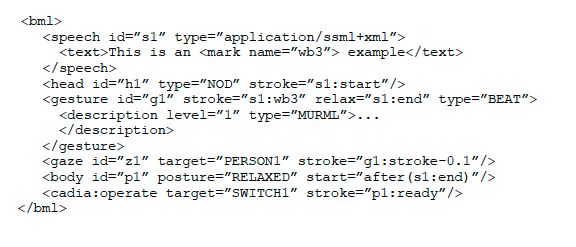
\includegraphics[width=\textwidth]{figures/bml-example.png}
\captionof{figure}{Extracted from \parencite{vilhjalmsson2007behavior} section 2, BML block example}

This specialized block serves as a coordinating mechanism for speech, gesture, gaze, head and body movements, consolidating them by including corresponding behavior elements within a singular encompassing element. Additional <bml> behavior elements encompass torso, face, legs, lips, and a wait behavior. Each behavioral directive undergoes a structured organization into six distinct animation phases, demarcated by sync-points that bear the names of associated motion transitions \parencite{vilhjalmsson2007behavior}.

The synchronization process involves seven key sync-points: start, ready, stroke-start, stroke, stroke-end, relax, and end. Achieving synchrony between behaviors is facilitated by aligning the sync-points of different behaviors, thereby orchestrating a seamless coordination of actions at specific points in time. In the aforementioned example, the head nod's most exertive phase, the stroke, precisely coincides with the designated sync-point, demonstrating the intricacies of temporal alignment within the BML framework \parencite{vilhjalmsson2007behavior}.

A recent augmentation to BML involves the incorporation of "levels of description," a feature designed to offer a more intricate portrayal of behaviors beyond the capabilities of the fundamental BML tags and attributes (see fig. 4.5). Specifically, the integration of a MURML type description for the gesture alongside the essential BML gesture element \parencite{vilhjalmsson2007behavior}.


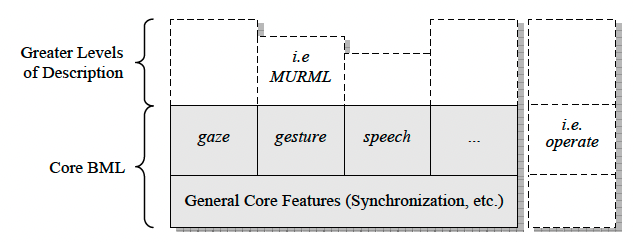
\includegraphics[width=\textwidth]{figures/bml.png}
\captionof{figure}{Extracted from \parencite{vilhjalmsson2007behavior} section 2, BML specification}

This approach aims to maintain the core BML specification entirely agnostic to animation engines, ensuring its independence while striking a judicious equilibrium between expressive detailing and streamlined efficiency. These additional levels provide an avenue for more nuanced or engine-specific depictions of behaviors already outlined in the core BML. This approach fosters flexibility and adaptability, enabling a richer and more detailed representation of behaviors without compromising the core specifications of BML \parencite{vilhjalmsson2007behavior}.




\section{Utterance syntesis}


\subsection{Sign inflections}

In sign language, the utterance synthesis process involves adapting sure signs' forms to reflect their context, known as sign inflection. There are two primary types of inflections. The first is due to sign language's illustrative or iconic nature, where gestures can resemble their meaning or function. The second type involves spatial referencing, which employs physical space to convey relational or locational information. Both inflections are critical for getting accurate and nuanced meanings in sign language \parencite{naert2020survey}.

\subsubsection{Iconic mechanisms}

Iconicity, defined as the presence of non-arbitrary connections between a language's form and meaning, is a distinctive feature of languages, particularly sign languages. Unlike spoken languages, where the relationship between sound and meaning is often arbitrary, sign languages exhibit a higher prevalence of iconicity. In sign languages, many signs bear a visible, intuitive connection to their intentions, making them more directly representational or illustrative of the concepts they convey. This aspect of sign languages highlights a unique dimension in which form and meaning are closely intertwined, offering insights into how different language modalities can structure communication \parencite{iconicityperlman}.

\textcite{naert2020survey} considered size and shape specifiers, classifiers, and role shifts as iconic mechanisms. 

\subsubsection{Spatial referencing}

\textcite{naert2020survey} presented two spatial referencing inflections, such as indicating verbs (see chap 2 section ) and pointing gestures, where pointing gestures involve using the hand, typically the tip of the index finger, to indicate a specific entity or location. These gestures serve multiple purposes: they can identify the subjects or objects of an action, such as in indications of 'I,' 'you,' or 'this one.'

\subsection{Concatenative}

Concatenative synthesis involves the sequential or simultaneous concatenation of pre-recorded or pre-synthesized motion segments across different Sign Language (SL) channels. Transitioning between these motion segments is achieved through motion interpolation or blending techniques. 
Motion blending specifically entails, at each frame, interpolating motions from the database to generate a new motion that preserves the characteristics of the initial motions. The foundation of motion synthesis lies in an annotated database of signs or more detailed motions, from which the system queries to compose the desired utterance. The quality of annotation plays a critical role; the annotation's granularity limits the synthesis's granularity, and the accuracy of data segmentation influences the presence or absence of artifacts in the final animation. The database, created and annotated offline, serves as the primary resource, while the concatenation of signs can be performed in real-time. This approach is particularly well-suited for utterance representations based on sequences of glosses. 

Some approaches use concatenative synthesis for utterance synthesis, such as Hand-Crafted Animations, Automatically Generated Signs, and MoCap Data.


Some research works that follow this approach are the avatars presented in \parencite{braffort2007demonstrations} and \parencite{paulaAvatar} 


\subsection{Articulatory Synthesis}

An alternative method for constructing sign language utterances involves generating them dynamically based on an utterance specification rather than relying on a predetermined database of static motion segments. This approach allows for the inclusion of iconicity, proforms, transitions between signs, and co-occurring phenomena directly within the sign description, enabling a more context-sensitive expression. According to \parencite{naert2020survey} only the GessyCA system \parencite{lebourque1999high} uses the articulatory synthesis alone to build utterances.
Constructing sentences in this manner offers precise control, but providing an utterance description using a sign or gesture specification (as the input for such a system) can be excessively laborious. Additionally, the resulting animation may lack realism and face potential rejection from the Deaf community \parencite{naert2020survey}.

Procedural methods for animating avatars based on sign representations are frequently employed, yet their extension to the utterance level is infrequently observed \parencite{naert2020survey}.


\subsection{Hybrid synthesis}

Hybrid models take advantage of the strengths of concatenative and articulatory synthesis. DePaul University research group implemented this idea on the avatar Paula \parencite{heloir2010real}, their avatar animated with hand-crafted keyframes \parencite{naert2020survey}.


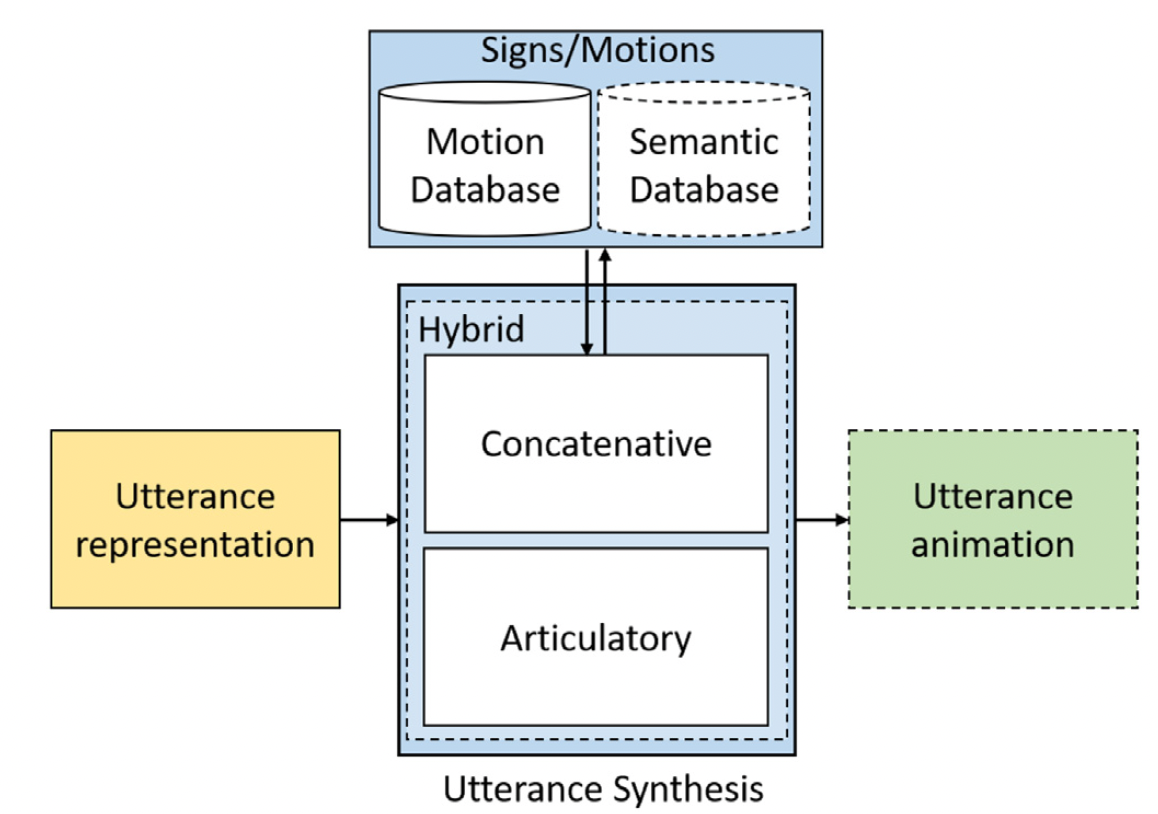
\includegraphics[width=\textwidth]{figures/utterancesynthesis.png}
\captionof{figure}{Extracted from \parencite{naert2020survey} section 5.2, utterance synthesis techniques }


\label{part:rrg}
%\thispagestyle{empty} % To avoid page numbers in blank pages
\chapter{Rol and Reference Grammar (RRG)}


The Role and Reference Grammar (RRG) stands as a significant theoretical framework in linguistics, playing a pivotal role in shaping the development of various linguistic theories, including Generalized Phrase Structure (Gazdar et al., 1985), Lexical Functional Grammar (LFG) (Bresnan, 1982, 2001), and Construction Grammar (Fillmore, 1988; Goldberg, 2006). Inspired by typological and theoretical considerations, this approach has left a lasting impact on linguistic scholarship, contributing to the exploration and understanding of diverse linguistic phenomena \parencite{van2009overview}.

\section{Sintactic structure}

The layered structure of a clause (LSC) is grounded in two essential distinctions: firstly, the differentiation between the predicate and non-predicating elements, and secondly, within the realm of non-predicating elements, the distinction between arguments and non-arguments (see Fig. 5.1). This distinction manifests in all languages, irrespective of their configurational nature, whether configurational or non-configurational, head-marking or dependent-marking, free-word-order or fixed-word-order. It encompasses the divide between noun phrases (NPs) and adpositional phrases that function as arguments of the predicate and those that do not \parencite{van1997syntax}. \\


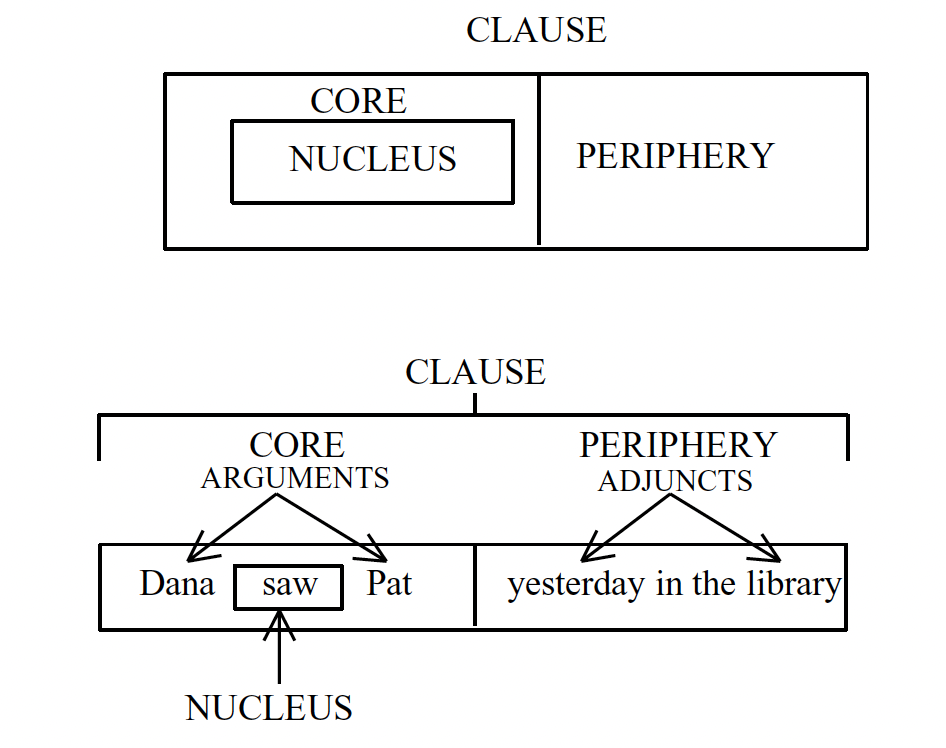
\includegraphics[width=\textwidth]{figures/clausestructure.png}
\captionof{figure}{Extracted from \parencite{van1997syntax} section 1.1, The layered structure of the clause }


In the English sentence, Dana saw Pat yesterday in the library; Dana saw Pat as the core (saw as the nucleus, Dana and Pat as the core arguments). And the library is on the periphery. The clause is divided into a core and a periphery. Within the core, a distinction is made between the nucleus (normally a verb) and its arguments (NPs and PPs, which are
arguments of the predicate in the nucleus). Core arguments are part of the semantic representation of the verb \parencite{van1997syntax}. The
relationships between the semantic and syntactic units are summarized in table 5.1\\

\begin{table}[H]
    \centering
    \begin{tabular}{|p{7cm}|p{4cm}|} \hline 
         \textbf{Semantic element(s)} &  \textbf{Syntactic unit}\\ \hline 
         Predicate & Nucleus\\ \hline 
         Argument in semantic representation of predicate& Core argument\\ \hline 
         Non arguments& Periphery\\ \hline 
         Predicate + arguments& Core\\ \hline 
         Predicate + arguments + Non- arguments& Clause (= core + periphery)\\ \hline
    \end{tabular}
    \caption{Relationships between the semantic and syntactic units}
    \label{tab:my_label}
\end{table}


The RRG (Role and Reference Grammar) conceptualization of the layered structure within a clause represents a semantically-driven perspective on non-relational syntactic structure. This theory posits that the foundational elements in the hierarchical arrangement of sentences and clauses derive their significance from semantic considerations, particularly the contrast between predicate and argument. Furthermore, it extends this semantic motivation to distinguish between XPs (e.g., NPs and PPs) associated with the predicate and those that are not. Thus, the layered structure is intricately shaped by the semantic interplay between predicate-argument relationships and the involvement of XPs concerning the predicate \parencite{van1997syntax}. \\

According to Van Valin (2005), a sentence may include a clause in a detached position, most commonly in the ‘left-detached position’ left [LDP]. This is the location of sentence-initial elements, most commonly adverbials, which are set off from the clause by a pause (See Fig. 5.2), e.g., Yesterday, I bought myself a new car. There is also a ‘right detached position’ [RDP], as in sentences like I know them, those boys. 
When the element in a detached position functions as a semantic verb argument, there is normally a resumptive pronoun in the core referring to it. \\

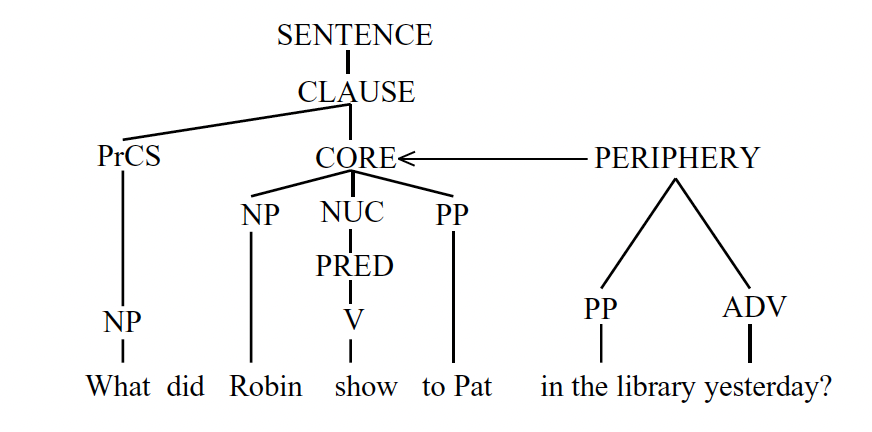
\includegraphics[width=\textwidth]{figures/completeclausestructure.png}
\captionof{figure}{Extracted from \parencite{van1997syntax} section 1.1, The structure of a English clause }

Question words, positioned immediately before the verb, are in the pre-core slot. Within this framework, the presence of an arrow signifies that the periphery functions as an optional modifier of the core.


The distinction between universal and non-universal aspects of clause structure unveils an intriguing observation. The universal elements, encompassing the nucleus, core, periphery, and the clause itself, are all grounded in semantic motivations \parencite{van1997syntax}.\\

In contrast, the non-universal facets, such as detached phrases and extra-core slots, lack semantic motivation; instead, their existence stems from pragmatic considerations \parencite{van1997syntax}. 


\subsection{Operators in the layered structure of a clause}

Grammatical categories such as aspect, tense, and modality are considered operators within the structure, influencing various layers of the clause. Each level of the clause can be subject to modification by one or more operators. The primary operators, or nuclear operators, exert influence over the nucleus, shaping the action, event, or state itself.

In Van Valin (2005), he proposed the following list of operators in LSC. 


\begin{table}[H]
    \centering
    \begin{tabular}{|p{4cm}|p{4cm}|p{4cm}|} \hline
         \textbf{Nuclear Operators} & \textbf{Core Operators} & \textbf{Causal Operators} \\ \hline 
         Aspects&  Directional & Status\\ \hline 
         Negation & Event Quantification & Tense\\ \hline 
         Directionals & Modals & Evidentials\\ \hline 
         &  Internal Negation & Illocutionary Force\\ \hline
    \end{tabular}
    \caption{Operators}
    \label{tab:operators}
\end{table}


Classifying a specific operator as nuclear, core, or clausal is directly determined by its meaning. It's important to note that not all languages necessarily incorporate all of these operators as grammatical categories; their presence depends on each language's linguistic characteristics and features. 
Among the operators, illocutionary force and negation are universal elements in every language. Clausal operators function to modify the entire clause, and they can be categorized into two groups. The first group comprises tense and status; the second includes evidentials and illocutionary force. Notably, negation is the sole operator across all three levels: nuclear, core, and clause.


\subsection{Formal Representation of Clause Structure}

The operators function as modifiers for the core, nucleus, and periphery, distinct from being integral components of these elements. They are represented independently, separate from the predicates and arguments they modify. The ordering of predicates and arguments is subject to language-specific constraints, while the primary guiding principle for arranging operators is the universal scope constraint. \\

Johnson (1987) proposed a formalization of the layered
structure of the clause in which predicates and their arguments are represented in a distinct projection from the one representing operators. This formalization
he termed a ‘projection grammar.’ The schematic depiction of the layered structure of a clause within a projection grammar is illustrated in Fig. 5.3

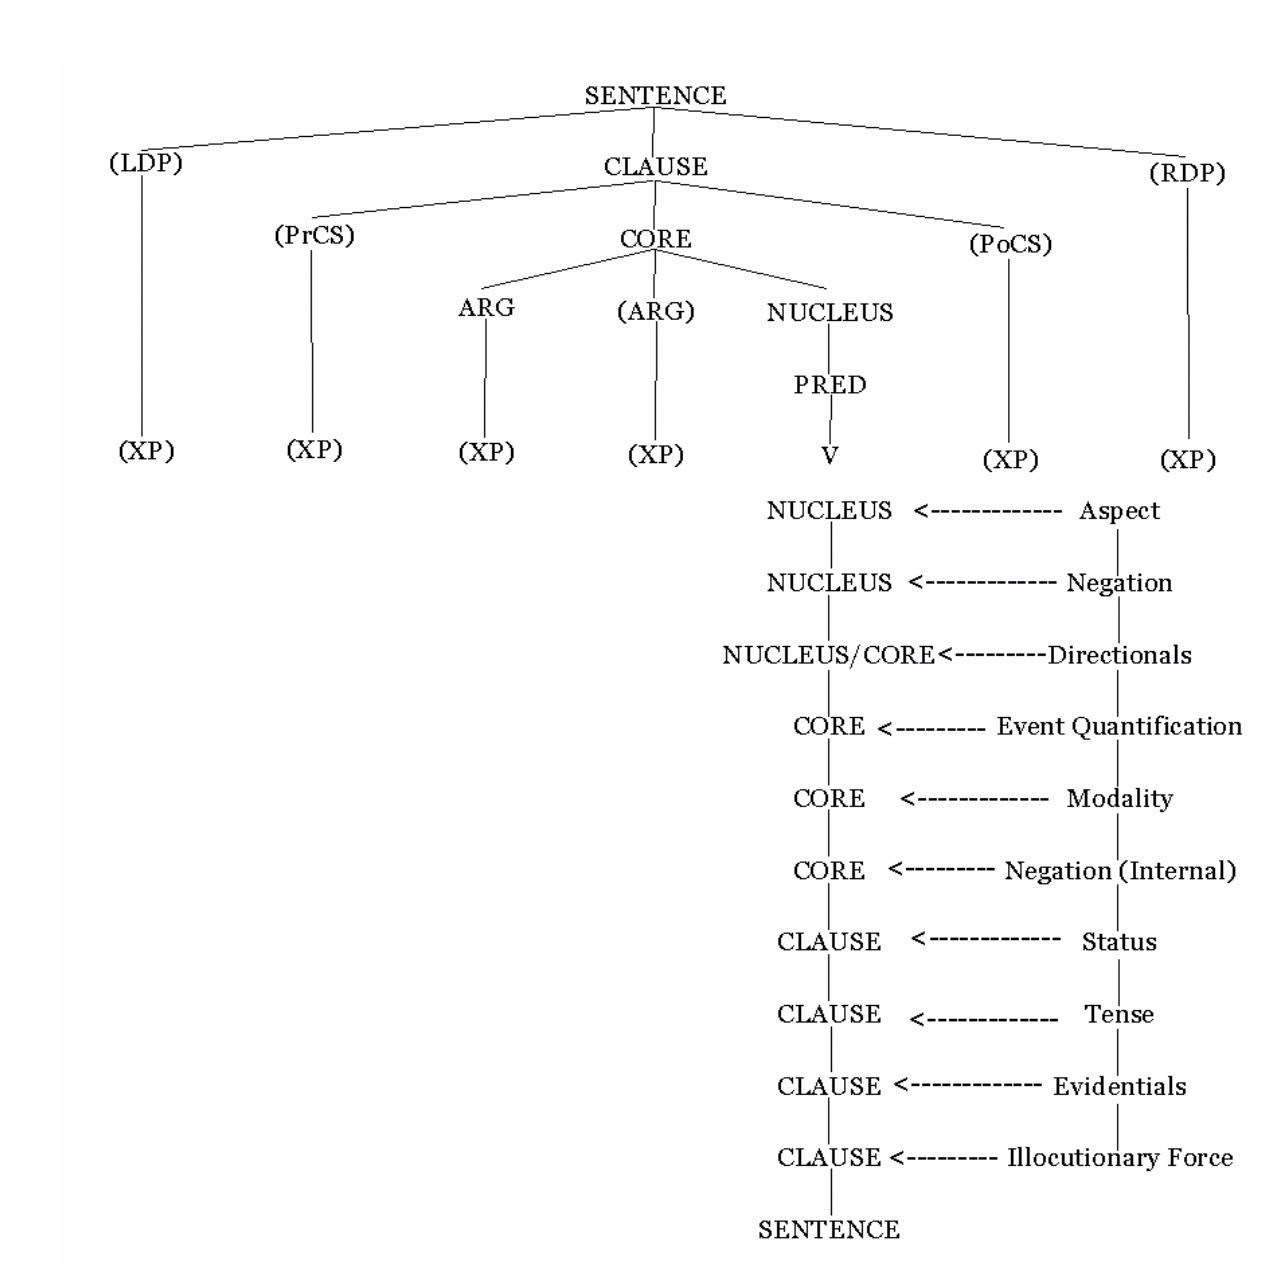
\includegraphics[width=\textwidth]{figures/general-structure-clause.png}
\captionof{figure}{Extracted from \parencite{van1997syntax} section 1.3, Layered structure of the clause with constituent and operator projections}

\subsection{Verb Classes}

In RRG originates from Vendler's (1967) Aktionsart-based categorization of verbs, which classifies them into states, achievements, accomplishments, and activities. RRG incorporates a modified version of Dowty's (1979) representational scheme.

States depict static situations that are inherently temporally unbounded (atelic), and achievements and accomplishments express changes of state, which
are inherently temporally bounded (telic): achievements are instantaneous, while accomplishments are not. Activities are dynamic, inherently temporally unbounded (atelic), states of affairs (\parencite{van1997syntax}).\\

The RRG verbs classification is based on the Aktionsart proposed by Vendler (1967) where verbs are categorized into states, achievements, accomplishments and activities. These four classes can be more precisely delineated by considering three features: [±static], [±punctual], and [±telic] (Binns-Dray, 2004). Static imply if a verb exhibits if something happening. If one answer the question ‘what happened?’ or ‘what is happening?’ then the verb is considered to be static. Telic pertains to whether a verb represents a state of affairs with an inherent terminal point. The last feature, 'punctual,' differentiates events with internal duration from those that lack it. Achievements and accomplishments are telic,or bounded. States and activities are atelic, or unbounded. \\

In addition to the verb classes there are two more,  active accomplishments, which describe telic uses
of activity verbs (e.g. devour), these verbs can be modified by adverbs, and on the other way semelfactives which sometimes describe if the situation involves an action or not (dynamic).\\

Below in table see examples of each class and their formal representation, including their causative counterparts.


\begin{table}[H]
    \centering
    \begin{tabular}{|p{3.5cm}|p{7.5cm}|} \hline 
         \textbf{Verb Classes} & \textbf{Examples}\\ \hline 
         State& be sick, be tall, be dead, love, know, believe, have\\ \hline 
         Activity& march, swim, walk (– goal PP); think, eat (+ mass noun/bare plural
RP)\\ \hline 
         Semelfactive& flash, tap, burst (the intransitive versions), glimpse\\ \hline 
         Achievement& pop, explode, shatter (all intransitive)\\ \hline 
         Acomplishment& melt, freeze, dry (the intransitive versions), learn\\ \hline 
         Active accomplishment& walk (+ goal PP), eat (+ quantified RP), devour\\ \hline
    \end{tabular}
    \caption{Examples of verbs of each class, taken from \textcite{van1997syntax}: 105, based on Example 3.21}
    \label{tab:my_label}
\end{table}



\begin{table}[H]
    \centering
    \begin{tabular}{|p{3.5cm}|p{7.5cm}|} \hline 
         Examples& Causative counterparts\\ \hline 
         State: The boy is afraid.& The dog frightens/scares the boy.\\ \hline 
         Achievement: The balloon popped.& The cat popped the balloon.\\ \hline 
         Semelfactive The pencil tapped on the table.& The teacher tapped the pencil on the table.\\ \hline 
         Accomplishment: The ice melted.& The hot water melted the ice.\\ \hline 
         Activity: The soldiers marched in the park.& The sergeant marched the soldiers in the park.\\ \hline 
         Active accomplishment: The soldiers marched to the park.& The sergeant marched the soldiers to the park.\\ \hline
    \end{tabular}
    \caption{Examples and causative counterparts, taken from \textcite{van2005exploring}: 34 Example 2.5}
    \label{tab:my_label}
\end{table}


\subsection{Lexical representation of verb classes}

An explanation for these patterns can be found in the lexical representations used in RRG: verbs are analyzed in terms of a lexical decomposition system in which state and activity predicates are taken as basic, and the other classes are derived from them.


\begin{table}[H]
    \centering
    \begin{tabular}{|p{3.3cm}  p{7.7cm}|}
     \hline
     \multicolumn{2}{|c|}{} \\ 
         \textbf{Aktionsart class} & \textbf{Logical structure} \\ [.3cm]
         State &  \textbf{predicate'} (x) or (x, y)  \\ [.3cm]
         Activity &  do' (x, [ \textbf{predicate'} (x) or (x, y)] \\  [.3cm]
         Achievement & INGR  \textbf{predicate'} (x) or (x, y), or INGR do' (x[ \textbf{predicate'}(x) or (x, y)])  \\ [.3cm]  
         Semelfative & SEML  \textbf{predicate'} (x) or (x, y) SEML do' (x, [ \textbf{predicate'}(x) or (x, y)]) \\  [.3cm]  
         Accomplishment & BECOME predicate' (x) or (x, y), or BECOME do' (x,[ \textbf{predicate'} (x) or (x, y)]) \\ [.3cm]  
         Active accomplishment & do' (x, [ \textbf{predicate1'} (x, (y))]) \& INGR  \textbf{predicate2'} (z, x) or (y) \\  [.3cm]  
         Causative & $\alpha$ CAUSE $\beta$, where $\alpha$, $\beta$ are logical structures of any type \\  [.3cm]
         \hline
    \end{tabular}
    \caption{Lexical representations for Aktionsart classes, taken from \textcite{van2005exploring} Section 2.1.2 Logical structures,  table 2.3}
    \label{tab:my_label}
\end{table}


These decompositional representations of verbs are referred to as 'logical structures,' the schemas for the classes can be found in Table 5.5. Adhering to the conventions of formal semantics, constants (typically predicates) are presented in boldface, followed by a prime. In contrast, variable elements are presented in normal typeface, often with a (+). The elements in boldface prime form part of the vocabulary of the semantic metalanguage used in the decomposition; they do not correspond to words from any specific human language. Therefore, the same representations are applicable across languages. For instance, the logical structure for Lakhota "t’´a" and English "die" would be "BECOMEdead(x)"  \parencite{van2005exploring}. \\


Examples of some English verbs with their logical structure are presented below in Example 5.2. 


\begin{enumerate}
    \item States
     \begin{enumerate}
        \item Pat is a fool. \\
              \textbf{be'} (Pat, [fool'])
         \item The cup is shattered. \\
         \textbf{shattered'} (cup)
         \item Kim is in the library.\\ 
         \textbf{be-in'} (library, Kim)
         \item Dana saw the picture.\\ 
         \textbf{see'} (Dana, picture)
    \end{enumerate}
    \item Activities
     \begin{enumerate}
         \item The children cried. \\ 
         \textbf{do'} (children, [cry' (children)])
         \item Carl ate pizza. \\
         \textbf{do'} (Carl, [eat'(Carl, pizza)])
     \end{enumerate}
     \item Achievements
     \begin{enumerate}
         \item The window shattered. \\ 
         INGR shattered' (window)
         \item The balloon popped. \\ 
         INGR popped' (balloon)
     \end{enumerate}
     \item Semelfactivities
     \begin{enumerate}
         \item  Dana glimpsed the picture. \\
         SEML see' (Dana, picture)
         \item Mary coughed. \\
         SEML do' (Mary, [cough' (Mary)])
     \end{enumerate}
    \item Accomplishments
     \begin{enumerate}
         \item The snow melted. \\
         BECOME melted' (snow)
        \item Mary learned French. \\ 
        BECOME know' (Mary, French)
     \end{enumerate}
    \item Active accomplishments
    \begin{enumerate}
         \item Chris ran to the park. \\
         do' (Chris, [run' (Chris)]) \& INGR be-at' (park, Chris)
        \item Carl ate the pizza. \\
        do´ (Carl, [eat' (Carl, pizza)]) \& INGR consumed' (pizza)
    \end{enumerate}
    \item Causatives
    \begin{enumerate}
        \item Max melted the ice. \\
        $[do' (dog, \Theta)] CAUSE [feel' (boy, [afraid'])]$  
        \item Max melted the ice. \\
        $[do' (Max, \Theta)] CAUSE [BECOME melted' (ice)]$
        \item The cat popped the balloon. \\
        $[do' (cat, \Theta)] CAUSE [INGR popped' (balloon)]$
        \item Sam flashed the light.  \\
        $[do' (Sam, Ø)] CAUSE [SEML do' (light, [flash' (light)])]$
        \item Felix bounced the ball. \\
        $[do' (Felix, Ø)] CAUSE [do' (ball, [bounce' (ball)])]$
        \item Mary fed the pizza to the child.\\
        $[do' (Mary, Ø)] CAUSE [do' (child, [eat' (child, pizza)])
        \& INGR consumed' (pizza)]$
    \end{enumerate}
\end{enumerate}


\subsection{Semantic roles}

In RRG, two categories of semantic roles, specific and general, are utilized. Specific semantic roles align closely with thematic relations proposed in other theories. The logical structure of a verb serves as a key indicator of its semantic properties, and these properties, as identified by Binns-Dray (2004), determine the corresponding thematic relations.

In addition, according to \textcite{van2005exploring}, the subsequent phase in RRG is refining the semantic representation, which involves defining the semantic relationships between a verb or another predicator and its corresponding arguments.\\

Semantic roles are explored at three distinct levels of generality. The first level encompasses specific roles tied to verbs: runner, killer, hearer, broken, and more. Thematic relations constitute the second level, offering generalizations across these verb-specific roles, including agent, instrument, experiencer, theme, and patient. The third level introduces generalized semantic roles, namely actor and undergoer, which extend across thematic relations \parencite{van2005exploring}. Based on these definitions, in (Example 5.2 1a), Pat is classified as an identified, serving as the first argument of an identificational predication. Meanwhile, the cup is identified as a patient, representing the singular argument in a one-place stative predicate denoting a state or condition. \\

The actor serves in a broad category encompassing roles like agent, experiencer, instrument, and others. In contrast, the undergoer serves as a generalization covering roles such as patient, theme, recipient, and more. The agent is the prototype for the actor, and the patient is the prototype for the undergoes. \\

In the RRG context, two essential semantic roles are proposed: thematic relations and semantic macro roles. These roles are pivotal in the linking system \parencite{van2005exploring}.


\subsubsection{Thematic relations}


\textcite{van2005exploring} states that thematic relations are delineated by referencing the argument positions within the decomposed logical structure representations, a framework influenced by Jackendoff's (1976) work.


\begin{table}[H]
\centering
\begin{tabular}{@{}lll@{}}
\hline
\multicolumn{3}{l}{I. STATES}                         \\
\hspace{2em}A. Single argument    &    &   \\
\hspace{4em}1. State or condition & broken'(x)    & x = patient   \\
\hspace{4em}2. Existence          & exist'(x)     & x = entity    \\
\multicolumn{3}{l}{\hspace{1.5em}B. Two arguments}                  \\
\hspace{4em}1. Pure location & be-LOC'(x, y) & x = location, \\ & & y = theme \\
  \hspace{4em}2. Perception   & hear' (x, y) & x = perceiver, \\ & &
y = stimulus            \\
    \hspace{4em}3. Cognition & know' (x, y) & x = cognizer,  \\ & &
y = content            \\
\hspace{4em}4. Desire & want' (x, y) & x = wanted, \\ & &
y = desire              \\
\hspace{4em}5. Propositional Attitude & consider' (x, y) & x = judged, \\& & y = judgment               \\
\hspace{4em}6. Possession & have' (x, y) & x = possessor, \\ & & y = possessed              \\
\hspace{4em}8. Emotion & love' (x, y) & x = emoter, \\ & & y = target \\
\hspace{4em}9. Attributive & be' (x, [pred']) & x = attributant, \\ & & y = attribute   \\
\hspace{4em}10. Identificational & be' (x, [pred']) & x = identified, \\ & & y = identity \\
\hspace{4em}11. Specificational & be' (x, y) & x = variable, \\ & &
y = value \\
\hspace{4em}12. Equational & equate' (x, y) & x, \\ & & y = referent \\
II. ACTIVITY VERBS  && \\
\hspace{2em}A. Single argument  && \\
\hspace{4em}1. Unspecified action & do' (x, Ø) & x = effector \\
\hspace{4em}2. Motion & do' (x, [walk' (x)]) & x = mover \\
\hspace{4em}3. Static motion & do' (x, [spin' (x)]) &  x = st-mover \\
\hspace{4em}4. Light emission & do' (x, [shine' (x)]) & x = l-emitter \\
\hspace{4em}5. Sound emission & do' (x, [gurgle' (x)]) & x = s-emitter \\
\hspace{2em}B. One or two arguments && \\
\hspace{4em}1. Performance & do' (x, [sing' (x, (y))]) & x = performer, \\ && y = performance \\
\hspace{4em}2. Consumption & do' (x, [eat' (x, (y))]) & x = consumer, \\ &&
y = consumed \\
\hspace{4em}3. Creation & do' (x, [write' (x,(y))]) & x = creator, \\ &&
y = creation \\
\hspace{4em}4. Directed perception & do' (x, [hear' (x, (y))]) & x = observer,  \\ && y = stimulus \\
\hspace{4em}5. Use & do' (x, [use' (x, y)]) & x = user, \\
&& y = implement \\
\hline
\end{tabular}
\caption{Thematic relations}
\label{tab:my-table}
\end{table}


Activity verbs constitute another category of primitive predicates featuring a minimum of ten subclasses. In non-motion activity verbs, the initial argument is an effector—an unmarked participant engaged in an action without specific indications of volition and control. Additional thematic relations linked to the first argument of activity verbs essentially function as subtypes of an effector. Although activity verbs typically prefer a single argument, some exceptions exist with a potential for two arguments, as seen in verbs like eat, drink, and play.


\subsubsection{Macroroles}

The second type of semantic role is the generalized semantic role, the
two macroroles, ‘actor’ and ‘undergoer.’ These constitute the two principal arguments within a transitive predication, and either one has the potential to function as the single argument in an intransitive verb. \\


Examples of actor and undergoer are illustrated below in Example 5.3. \\

\begin{enumerate}
    \item $[\textbf{do'} (Pat, \theta)] \hspace{1em}CAUSE [BECOME \hspace{1em}\textbf{have'} (Chris, book)]$
    \item Pat [actor] gave the book [undergoer] to Chris.
    \item Pat [actor] gave Chris [undergoer] the book.
\end{enumerate}

\textcite{van2005exploring}:61 Example 2.40 \\

The actor represents the argument most akin to an agent, and the undergoer embodies the most reminiscent of a patient. Termed 'macroroles,' these designations encompass various specific thematic relations (See Fig. 5.4). The rationale behind macroroles lies in the observation that grammatical constructions often treat groups of thematic relations similarly.\\

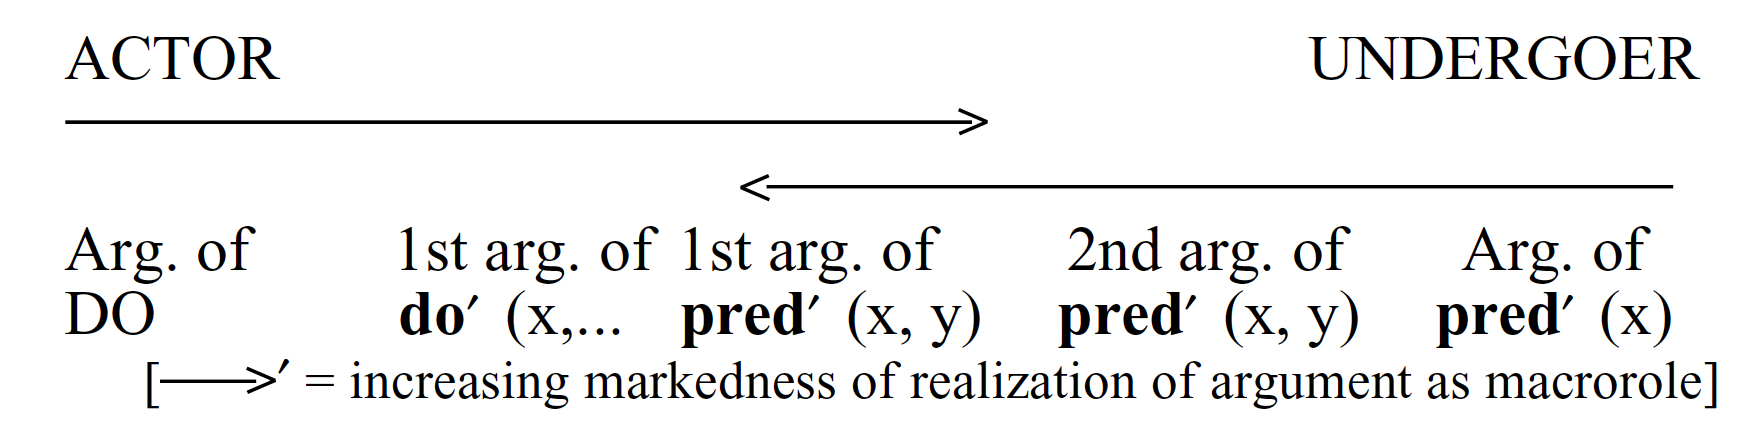
\includegraphics[width=\textwidth]{figures/macroroles-hierarchy.png}
\captionof{figure}{Extracted from \parencite{van2005exploring} section 2.4.2, Actor–undergoer hierarchy (preliminary)} \hfill


The connection between macroroles and logical structure argument positions is encapsulated in the actor-undergoer hierarchy. This principle straightforwardly asserts that, within the logical structure of a transitive verb, the actor is identified as the leftmost argument, while the undergoer is positioned as the rightmost argument.


\section{The Linking System}

The RRG linking algorithm is bidirectional. It establishes a connection between the meaning and structure of language, linking semantic representation to syntactic representation and vice versa.  \\


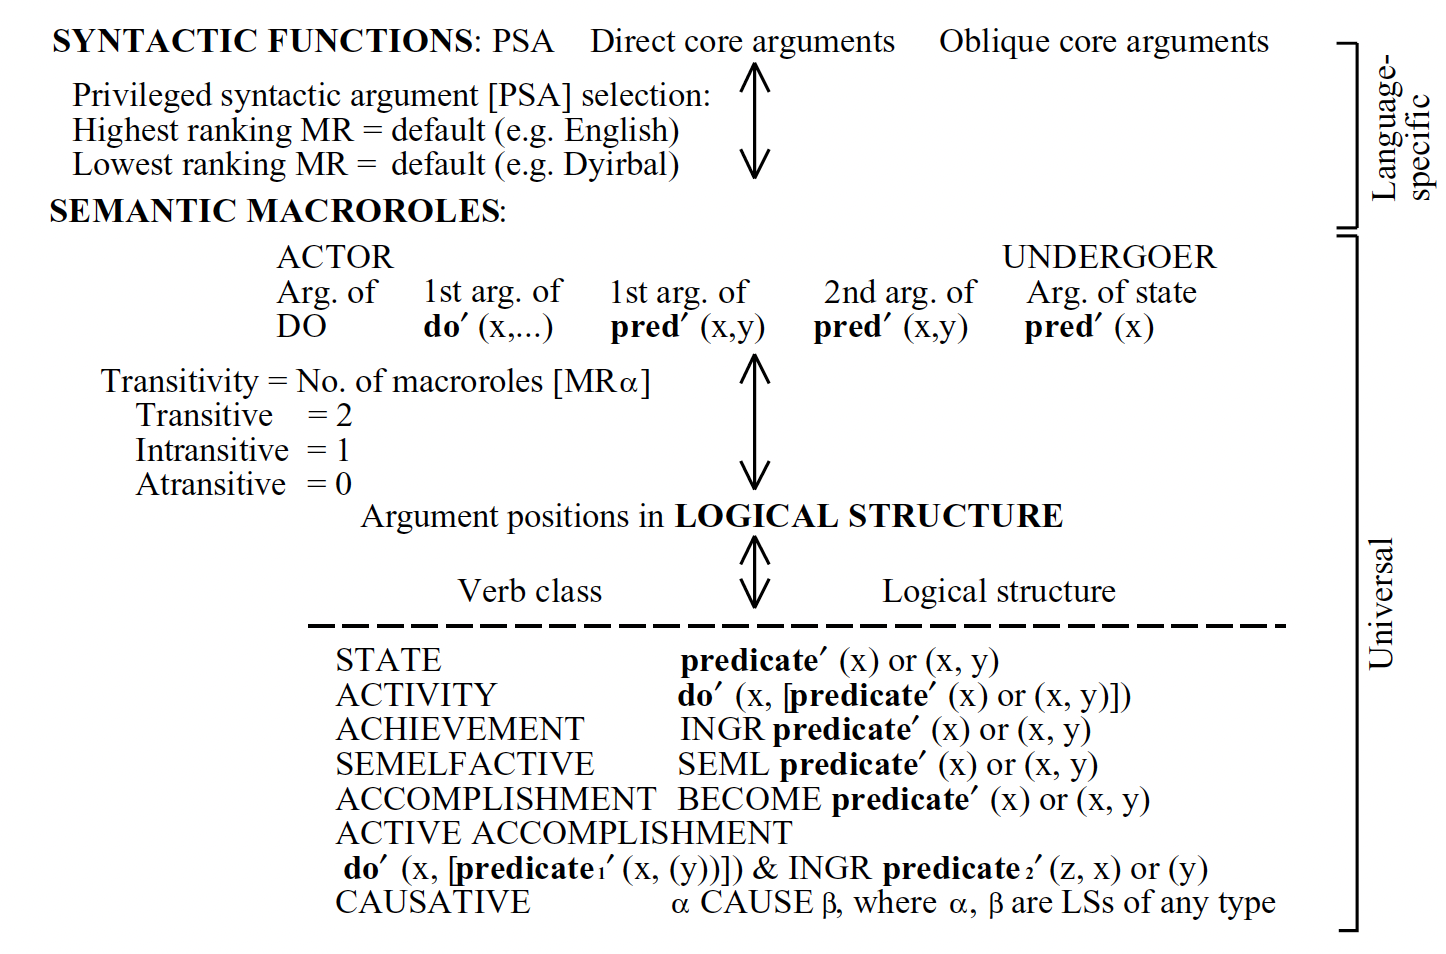
\includegraphics[width=\textwidth]{figures/linking-algorithm.png}
\captionof{figure}{Extracted from \parencite{van2005exploring} section 5.1, Linking algorithm}


Example 5.3 

\begin{enumerate}
    \item Step 1: Construct semantic representation in Lexicon.
    \begin{enumerate}
        \item Access LS for sitting and select prepositional LS to fill be-LOC´ slot in LS, on: \\
        $do' (x sit´ (x, [be-LOC' (y, x)]) + be-on' ( , )]) \\ \implies$
        $do' (x [sit' (x, [be-on' (y, x)])])$
        \item Determine the value of the operators to be expressed:\\
        $<IF DEC <TNS PRES < do' (x, [sit' (x, [be-on' (y, x)])])>>>$
        \item Select the referring expressions to fill the variable positions in LS: \\
        $<IF DEC <TNS PRES < do' (Book, [sit' (Book, ([be-on' (Table, Book))])>>>$
    \end{enumerate}
    \item Step 2: Determine actor and undergoer assignments:\\
    $<IF \hspace{1em} DEC \hspace{1em} <TNS \hspace{1em} PRES < do' (ACT: Book, [sit' (Book, [be-on' (Table, Book)])])>>>$
\item Step 3: Determine the morphosyntactic coding of the arguments:
     \begin{enumerate}
         \item PSA selection: Actor as sole macrorole is selected as PSA.
          \item Actor is assigned nominative case as highest ranking macrorole; 
                preposition on is assigned to the table, which receives dative case due to being the first argument of be-on´, a static location.
          \item As the tense is present, the agreement marking is on the nucleus. The nucleus will agree with the actor since it is the highest ranking macrorole.
     \end{enumerate}
\item Step 4: Select syntactic templates:\\
    \begin{enumerate}
         \item Select the PrCS template, which is obligatory in main declarative clauses.
          \item d. n. a.
           \item Select a two-place core, one place for the nucleus and one for the PP.
            \item Select the non-branching nucleus template.
             \item Select two common noun NP templates and a predicative PP template.
    \end{enumerate}
\item Step 5: Assign LS elements to positions in the syntactic representation:
    \begin{enumerate}
         \item Assign the predicate to the nucleus.
         \item Join the operator projection template to the nucleus and attach the
            morphemes expressing operators to it.
         \item (1.a). Since the nucleus is finite, link it to the first position in the core.
         \item Link the nominative case-actor The Book to the PrCS.
         \item Link the PP to the remaining core position.
\end{enumerate}
\end{enumerate}

\section{Sign\_A framework}

The Sign\_A framework, proposed by \parencite{murtagh2019linguistically}, addresses the absence of a universally accepted standard for documenting Sign Languages (SLs). Developed to facilitate the inclusion of sign languages in the SL lexicon, the framework introduces the 'Articulatory Structure Level' (A). This level, known as the Articulatory Structure Level, expands upon the generative lexicon (GL) theory proposed by Pustejovsky in 1991. \\

Pustejovsky (1995) describes the Generative Lexicon (GL) as a linguistic semantics theory emphasizing the decentralized nature of compositionality in natural language. The GL theory has four main levels of representation. as follows: 


\begin{table}[H]
    \centering
    \begin{tabular}{|p{4cm}|p{7cm}|} \hline 
         Lexical representation level& Description\\ \hline 
         Argument structure& The behavior of a word as a function, with
its arity specified. This is the predicate
argument structure for a word, which
indicates how it maps to syntactic
expressions.\\ \hline 
         Event structure& Identification of the particular event type
(in the sense of Vendler (1967)) for a
word or phrase: e.g., as state, process, or
transition.\\ \hline 
         Qualia structure& The essential attributes of an object as
defined by the lexical item.\\ \hline 
         Inheritance structure& How the word is globally related to other
concepts in the lexicon..\\ \hline
 Articulatory Structure&The essential (computational) phonological
parameters of an object as defined by the lexical
item.\\\hline
    \end{tabular}
    \caption{Five levels of lexical representation for Sign Language Murtagh (2019)}
    \label{tab:my_label}
\end{table}


A fifth level of lexical representation incorporates an object's essential (computational) phonological parameters as defined by the corresponding lexical item. These parameters play a pivotal role in capturing the computational phonological essence of an object. They will be instrumental in addressing diverse linguistic phenomena related to the ISL manual and Non-Manual Features (NMFs). This inclusion is imperative for comprehensively representing ISL within a computational framework \parencite{murtagh-etal-2022-sign}. \\


In contrast, the non-universal facets, such as detached phrases and extra-core slots, lack semantic motivation; instead, their existence stems from pragmatic considerations.



\chapter{Creating an Avatar}

This section is for building a 3D avatar using a specific group of software tools.

\section{Signing Avatar Development Technologies}


Unity is a cross-platform graphics engine developed by Unity Technologies, specializing in creating 2D and 3D video games and audio and animation rendering. This engine offers networking tools for multiplayer experiences, NavMesh navigation tools for Artificial Intelligence, Virtual Reality support, and real-time interactive content creation. Based on the C\# programming language, Unity brings graphics to life in the game. Its robust documentation and active user community are remarkable, providing resources and support for developers. For Windows, Mac OS, and Linux, Unity has been widely used in various games thanks to its versatility in adapting to different systems, creating 2D and 3D scenes with real-time animations and high-quality graphics performance, and providing an immersive experience. Unity offers both a free and a paid version with more advanced features.\\

MakeHuman is a user-friendly tool crafted to integrate the process of building virtual human characters through a Graphical User Interface (GUI). MakeHuman aims to simplify and enhance the creation of lifelike virtual humans, providing an efficient approach to this particular branch of digital design. \\

Ready Player Me accommodates full and half-body avatars, specifically optimized to enhance real-time game performance and uphold quality standards. This adaptable avatar system is crafted for games, VR/AR experiences, and applications. Furthermore, it seamlessly aligns with various technologies and game engines, including Unity, Unreal Engine, React, native mobile solutions, and API integration with stacks supporting REST and PostMessage protocols. Incorporating the Ready Player Me Avatar creator into your application or game is user-friendly. With many customization options, users can personalize avatars to reflect their identities genuinely. These avatars are supplied fully skinned, rigged, and primed for animation, ensuring a smooth integration into the preferred development environment. For a streamlined integration experience, developers can leverage the provided SDKs (Unity, Unreal, React) or engage directly with the APIs and/or iFrame Avatar Creator integration. The Ready Player Me avatar system functions as an all-encompassing solution for creating, managing, integrating, and customizing player avatars across diverse platforms, encompassing web, desktop, mobile, VR, and others supported by Unity and Unreal Engine. \\


Blender stands out as a comprehensive, free, and open-source 3D creation suite that spans the entire spectrum of the 3D pipeline. This includes modeling, rigging, animation, simulation, rendering, compositing, motion tracking, video editing, and even game creation. Operating as a cross-platform application, Blender seamlessly functions on Linux, Windows, and Macintosh computers. Its interface, powered by OpenGL, ensures a consistent and user-friendly experience.

With Blender, users can unleash their creativity to generate diverse 3D visualizations encompassing still images, 3D animations, and VFX shots. The software is built on a high-quality 3D architecture, facilitating a speedy and efficient workflow for content creation.

What sets Blender apart is not only its robust features but also its vibrant community support. Users benefit from an active community that contributes to ongoing improvements, making Blender a powerful and accessible tool for 3D enthusiasts across the globe. 

Blender is considered as a tool for this research as it
provides several features as mentioned before that will support in the development of an embodied conversational agent. Blender provides its avatar rendering engine, which
provides capabilities for real-time processing. 
\label{part:avatartech}

%%================================================================%
%% Bibliography
%%================================================================%
%\newpage
%\thispagestyle{empty} % To avoid page numbers in blank pages
\cleardoublepage\addcontentsline{toc}{chapter}{Bibliography}

% Choose citation styles depending on whether you want numeric/alphabetic in settings.tex
\printbibliography
%================================================================%
% Appended papers
%================================================================%
%The actual papers that are included in the thesis





%
%================================================================%
% Appendices
%================================================================%
%\cleardoublepage
%I place all appendices at the end of the thesis. Of course, you can also change this so that each appendix is directly following the paper it belongs to.
%\addcontentsline{toc}{chapter}{Appendix}
%\appendix
%\chapter{Appendix - Paper A}
%\section{Data Collection Instruments}
\label{paperB:instrument}
\begin{enumerate}
 \item Nothing!
 \item Nothing!
\end{enumerate}


\end{document}
